\documentclass[11pt]{article}
\usepackage[margin=1in]{geometry}
\usepackage{booktabs,amsmath,amssymb,enumitem,tabularx,graphicx,float}
\usepackage[hidelinks]{hyperref}
\graphicspath{{../shared/results/paper2_6_hybrid_pra/}{../shared/results/paper2_6_hybrid_pra/channel_geometry/}{../shared/results/paper2_6_hybrid_pra/channel_selection/}{../shared/results/paper2_6_hybrid_pra/channel_selection/normalized_efficiency/}{../shared/results/paper2_6_hybrid_pra/final_iteration/}{../shared/results/paper2_6_hybrid_pra/indexed_confirmation/}{../shared/results/paper2_6_hybrid_pra/end_to_end_confirmation/}{../shared/results/paper2_6_hybrid_pra/interaction_confirmation/}}
\setlength{\emergencystretch}{3em}
\title{Retrieval Representation and Native-State Consumption Under a Bounded Memory Budget}
\author{Jorge Simao\\EInnovator R\&D -- Center for the Sciences of Computation, Cognition, and Complexity}
\date{\today}
\begin{document}
\maketitle

\begin{abstract}
Progressive Retrieval Attention (PRA) exposes a logical memory while admitting a bounded native key/value working set. We ask which representation should retrieve the identities to admit, comparing contextual semantic gists, exact model-token identity, BM25, approximate matching, and hybrid search. The primary evaluation is an annotation-constructed mechanism benchmark: evidence strings are prepended to a 1,536-token source before retrieval. A same-budget first-four positional control consequently reaches 0.990--0.995 HotpotQA and 0.954 QASPER evidence recall, above every routed channel; these results do not establish ordinary document retrieval. Within this controlled setting, BM25 leads held-out HotpotQA and approximate matching leads QASPER for both tested model/tokenizer families on the same 50 questions per dataset. The learned ensemble remains below a validation-selected fixed channel in three of four panels. A posting-list prototype matches exhaustive Top-4 on all 96 synthetic scaling queries while scoring about one tenth of rows, but its 68.4x mean routing speedup is relative to the matching Python exhaustive implementation and its semantic reserve still requires full-corpus scores. After selected identities enter a matched four-layer native-K/V materializer, Qwen HotpotQA semantic memory improves gold-answer token likelihood over disabled, shuffled, and irrelevant controls; generated-F1 improvement remains unresolved. On QASPER, evidence retrieval is high but routed likelihood gains over disabled memory remain unresolved, although oracle memory beats irrelevant memory. Retrieval success and useful frozen-model consumption are therefore separate empirical questions.
\end{abstract}

\section{Introduction}
An addressable memory is useful only if the system can find the right address. A semantic retriever can recognize that two passages discuss related ideas, but relatedness is not identity. The string \texttt{CVE-2026-1234}, a DOI, a URI, or a filename may identify one object exactly. An alias such as ``IBM'' may identify the same organization as ``International Business Machines.'' A question such as ``Which university did the founder of company X attend?'' instead asks for a relation whose answer need not repeat the question's words. These cases motivate the boundary
\[
\boxed{\text{semantic relatedness}\neq\text{referential identity}}.
\]

PRA treats long context as logical memory rather than requiring every source token to remain active at every decoding step~\cite{simao2026position,simao2026pra}. A compact representation first discovers candidate memory objects; a materializer then admits bounded native K/V; finally, the frozen model must use that state. This paper studies the first step and tests its handoff to the other two. It does not assume that higher retrieval recall implies better answers.

Consider a two-hop query with an evidence path
\[
Q\rightarrow C_1\rightarrow C_2.
\]
The root $C_1$ might be semantically related to the question. Once admitted, however, it may expose the exact name or identifier of $C_2$. The useful search representation can therefore change with state:
\[
S_{\mathrm{root}}\neq S_{\mathrm{succ}}.
\]
The same distinction separates this work from static sparse--dense fusion. We do not propose hybrid information retrieval as a novelty. We ask which retrieval representation should address identity-aligned PRA memory at each stage, whether those choices can be indexed sparsely, and whether the selected memory produces a causal effect after native-K/V admission.

The paper answers four questions within this annotation-constructed mechanism setting. First, measured semantic, exact, BM25, and approximate channels recover different evidence, but a positional first-four control exposes the shortcut created by evidence front-loading. Second, channel ordering repeats across two tested model/tokenizer families evaluated on the same held-out questions; this is model replication on a shared task sample, not two independent samples. Third, posting-list candidate generation empirically preserves Top-4 retrieval in the synthetic scaling suite while touching about 10\% of rows during final channel scoring. Fourth, routed HotpotQA memory produces likelihood effects under specific controls, whereas QASPER demonstrates that high retrieval recall can coexist with unresolved fixed-channel consumption.

Our contributions are:
\begin{enumerate}[leftmargin=*]
\item a multi-representational PRA discovery formulation that separates semantic relatedness from token and reference identity;
\item a controlled, annotation-constructed comparison of retrieval representations, including a positional baseline that reveals the construction's substantial front-loading advantage;
\item shared-question model replication of channel heterogeneity, with paired question-level uncertainty and an explicit negative result for the tested adaptive ensemble;
\item sparse indexed candidate generation that preserves measured Top-4 behavior on a synthetic scaling suite while substantially reducing work relative to its Python exhaustive implementation;
\item a matched native-K/V evaluation showing routed-content HotpotQA likelihood effects and a QASPER retrieval-to-consumption counterexample, without a generated-answer gain;
\item root/successor and interaction evidence showing dependence on stage, budget, granularity, and model; and
\item a versioned retrieval-action and provenance interface for downstream adaptive control.
\end{enumerate}

\section{PRA Memory Discovery}
PRA separates three questions that ordinary retrieval pipelines often conflate:
\begin{enumerate}[leftmargin=*]
\item \emph{Discovery}: which logical memory object is relevant?
\item \emph{Materialization}: which native K/V, at which layers and detail, enters the bounded working set?
\item \emph{Consumption}: does the model use that admitted state beneficially?
\end{enumerate}
Figure~\ref{fig:architecture} shows the experimental boundary. Logical sources are chunked and indexed once. A query chooses a retrieval representation, sparse candidate generation narrows the logical address space, and exact scoring returns stable identities. The inherited materializer resolves those identities to native K/V under a physical token budget. The frozen model then supplies a separate consumption measurement.

\begin{figure}[H]
\centering
\setlength{\fboxsep}{7pt}
\begin{tabular}{c}
\fbox{\parbox{.84\linewidth}{\centering Large logical memory: source objects, stable URIs, aligned token spans, and semantic gists}}\\[5pt]
$\downarrow$\\[-1pt]
\fbox{\parbox{.84\linewidth}{\centering Representation action: semantic, exact token identity, BM25, approximate token match, or hybrid/state-dependent search}}\\[5pt]
$\downarrow$\\[-1pt]
\fbox{\parbox{.84\linewidth}{\centering Sparse candidate union $\mathcal U(q)$ $\rightarrow$ exact channel scoring $\rightarrow$ selected logical identities}}\\[5pt]
$\downarrow$\\[-1pt]
\fbox{\parbox{.84\linewidth}{\centering Native-K/V materializer: matched chunk and physical-token budget across selected consumption layers}}\\[5pt]
$\downarrow$\\[-1pt]
\fbox{\parbox{.84\linewidth}{\centering Frozen-model consumption: gold-answer likelihood, generated EM/F1, causal controls, and physical accounting}}
\end{tabular}
\caption{Discovery, materialization, and consumption are separate interfaces. Paper~2.6 changes the representation used to discover logical identities, holds native-K/V materialization fixed in the held-out mechanism evaluation, and then measures whether the frozen consumer benefits.}
\label{fig:architecture}
\end{figure}

For evaluation, let $E$ be the nonempty set of required evidence-span identities, $S$ the deduplicated selected chunk identities, $I(S)\subseteq E$ the evidence spans intersected by $S$, and $H(S)\subseteq S$ the selected chunks intersecting any evidence span. We report
\[
R_E=\frac{|I(S)|}{|E|},\qquad
P_E=\frac{|H(S)|}{|S|},\qquad
C_E=\mathbf 1[I(S)=E].
\]
The loaders exclude empty-evidence examples. Metrics map each annotation string to its first exact occurrence in the constructed source; selected chunk identities are deduplicated before scoring. Candidate-normalized cost is reported separately as $|S|/N$, where $N$ is the logical candidate count, and $|S|/|E|$, the selected working-set overhead relative to required evidence. We never substitute candidates scored for chunks selected, physical K/V tokens, layer-token states, or wall-clock time.

\section{Retrieval Representations}
Table~\ref{tab:representations} summarizes the primary actions. All channels return stable row identities and retain provenance. The semantic channel scores a contextual query $q_{t,\ell}$ against layer-aligned chunk gist $g_{i,\ell}$,
\[
s^{\mathrm{sem}}_{i,\ell}=\cos(q_{t,\ell},g_{i,\ell}).
\]
Exact token spans preserve literal identity. BM25 rewards informative decoded terms. Approximate matching uses character-trigram candidate narrowing before bounded sequence comparison. Hybrid search can combine channels or choose different representations at root and successor stages. Explicit registered URIs form a deterministic product path when a caller already possesses the address; they are not a learned or oracle result.

\begin{table}[H]
\centering
\small
\caption{Primary retrieval representations and their characteristic strengths and failures.}
\label{tab:representations}
\begin{tabularx}{\linewidth}{lXX}
\toprule
Representation & Useful signal & Characteristic failure\\
\midrule
Semantic gist & contextual topic and implicit relation & literal identifiers can be blurred\\
Exact token & literal span, URI, filename, numeric ID & paraphrase, typo, and changed segmentation\\
BM25 & several moderately informative lexical terms & vocabulary mismatch and implicit relation\\
Approximate token & typo, partial mention, surface variation & collisions, stale aliases, wrong instance\\
Hybrid/stateful & complementary channels and newly exposed state & distractor dilution and score calibration\\
\bottomrule
\end{tabularx}
\end{table}

The token-native sidecar uses the host tokenizer rather than a second tokenizer vocabulary. It stores raw token IDs, normalized pieces, token $n$-grams, character trigrams, stable URIs, and row-aligned source offsets. BM25 nevertheless adds a lexical term layer: model tokens are decoded, word terms are normalized, and corpus document frequencies are maintained. Unicode NFKC and case folding repair compatibility forms, while aliases can come from headings, parenthetical names, or an application registry. Bounded token edit distance and mean host-input-embedding similarity are diagnostic extensions rather than silent defaults.

\subsection{Sparse Indexed Candidate Generation}
Exhaustive Python scoring makes routing cost proportional to the full logical memory even when only a few rows share query evidence. The indexed path instead constructs a deduplicated candidate union
\[
q\rightarrow\mathcal U(q)=
\mathcal P_{tok}\cup\mathcal P_{ngram}\cup\mathcal P_{bm25}
\cup\mathcal P_{char}\cup\mathcal P_{uri},
\qquad |\mathcal U(q)|\ll N,
\]
then applies the requested channel only inside the bounded pool. A reserved semantic slice prevents lexical postings from removing every semantically plausible row. Stable identities deduplicate cross-channel unions before ranking.

Across 256, 1,024, and 4,096 synthetic chunks and both tokenizers, a 64-row pool reproduces exhaustive Top-4 output on all 96 templated identifier-query comparisons. This is empirical parity on the measured suite, not a guarantee for arbitrary queries or corpora. Averaged over the suite, the indexed path sends 9.99\% of rows to final channel scoring and is 68.36x faster than the matching exhaustive Python implementation. The percentage excludes posting collection and semantic-score production: the current reserve receives a full semantic score vector and sorts it to retain semantically plausible rows. At 4,096 chunks, exact lookup falls from 33.6--37.0~s to 119--125~ms, a 283--300x prototype speedup. Weighted, approximate, and cascade paths improve by 56--64x but still take 0.50--0.65~s per query. These timings exclude model inference and are not comparisons with a production search engine.

\begin{figure}[H]
\centering
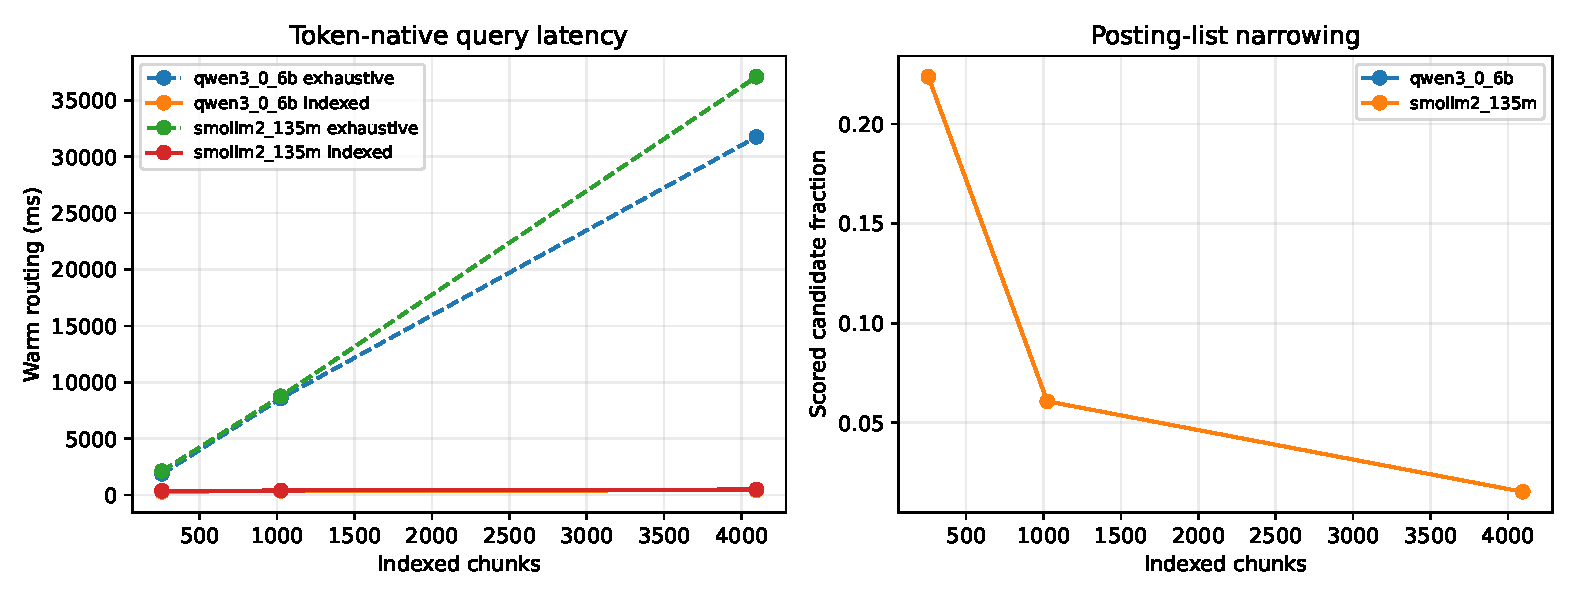
\includegraphics[width=.88\linewidth]{indexed_token_native_latency.pdf}
\caption{Exhaustive and indexed routing latency. Posting-list candidate narrowing keeps the scored pool bounded as logical memory grows. Exact lookup scales well in this prototype; fuzzy paths remain too slow for serving claims.}
\label{fig:indexed-latency}
\end{figure}

The immutable index rebuilds corpus statistics when references are added. At 4,096 chunks, cold construction takes 3.37~s for Qwen and 2.76~s for SmolLM; adding 64 chunks by full-statistics rebuild takes about 0.80~s. Warm lookup is reported separately. The index's estimated serialized payload is 10.06 and 10.94~MiB, excluding Python-object overhead and the external semantic-score computation. Appendix~\ref{app:index} gives the detailed timing and implementation contract.

\section{Held-out Retrieval and Consumption Evaluation}
\subsection{Protocol}
The campaign recorded as Gate B is the primary HotpotQA/QASPER mechanism evaluation. It uses Qwen3-0.6B and SmolLM2-135M with identities disjoint from the earlier discovery cohort. For each dataset, 20 examples tune only observable selector parameters and 50 fresh examples form the held-out test. Both model families evaluate the same questions. A serialized audit confirms no overlap among the four identity groups in Table~\ref{tab:cohorts}.

\begin{table}[H]
\centering
\scriptsize
\caption{Identity groups covered by the serialized overlap audit. Counts combine HotpotQA and QASPER equally. Model rows reuse the same question identities.}
\label{tab:cohorts}
\begin{tabularx}{\linewidth}{lrr>{\raggedright\arraybackslash}X>{\raggedright\arraybackslash}X}
\toprule
Group & IDs & Per dataset & Use and construction & Models / seeds\\
\midrule
Legacy exclusion & 48 & 24 & overlap guard for prior HotpotQA/QASPER work & Qwen; data seed 20260811\\
Validation & 40 & 20 & annotation-first; observable selector tuning & both models; data seed 20260823, five controller seeds\\
Held-out test & 100 & 50 & annotation-first; retrieval and consumption endpoints & both models; data seed 20260823\\
Interaction & 16 & 8 & annotation-first; descriptive configuration grid & both models; data seed 20260823\\
\bottomrule
\end{tabularx}
\end{table}

The mechanism construction places deduplicated annotated evidence strings first, appends the original source, bounds the result to 1,536 tokens, and partitions it into 32-token chunks. This only deduplicates the prepended list; evidence generally remains duplicated inside the appended source. Gold labels do not enter fixed or learned channel scores, but they determine source construction and metric locations, so this is not an unmodified QA benchmark. A tokenization-only audit finds that a same-budget first-four-chunk control already recovers .990--.995 HotpotQA evidence and .954 QASPER evidence. Literal evidence duplication remains in 48--50 of 50 examples per panel. Thus the experiment compares mechanisms under favorable annotation-constructed evidence placement; original-order, randomized-location, and fully deduplicated-source conditions remain unperformed.

Every routed condition receives four chunks, at most 128 unique native-K/V tokens, and the same four late consumption layers. Disabled and empty controls admit no external PRA memory; shuffled and irrelevant controls preserve the memory budget with wrong content. Bounded direct context places the source in the ordinary prompt and is neither compute nor quality matched. The oracle is an annotated ceiling.

\subsection{Shared-Question Retrieval Differences}
Table~\ref{tab:gateb-retrieval} gives the complete fixed-channel comparison and the positional construction control. Among routed methods, dataset-level ordering repeats across two model/tokenizer families on the same questions: BM25 leads HotpotQA at 0.665 and 0.662 recall, whereas approximate matching leads QASPER at 0.747 and 0.783. Paired winner-minus-semantic intervals exclude zero in all four panels (Table~\ref{tab:paired-retrieval}), but the winners were identified descriptively on held-out means and the intervals do not remove that post-selection caveat. The five-seed validation-trained ensemble remains below the strongest fixed channel; this architecture exposes representation choice but has not demonstrated a successful runtime selector.

\begin{table}[H]
\centering
\small
\caption{Annotation-constructed held-out evidence recall, 50 shared question identities per dataset and model. Bold marks the best routed fixed channel; Pos.-4 selects the first four chunks without retrieval. All conditions use at most four chunks.}
\label{tab:gateb-retrieval}
\resizebox{\linewidth}{!}{%
\begin{tabular}{llrrrrrrr}
\toprule
Model & Dataset & Semantic & Exact & BM25 & Approx. & Hybrid & Adaptive & Pos.-4\\
\midrule
Qwen & HotpotQA & .473 & .482 & \textbf{.665} & .593 & .505 & .543 & .995\\
Qwen & QASPER & .364 & .619 & .228 & \textbf{.747} & .457 & .576 & .954\\
SmolLM & HotpotQA & .320 & .450 & \textbf{.662} & .593 & .422 & .518 & .990\\
SmolLM & QASPER & .348 & .609 & .328 & \textbf{.783} & .437 & .446 & .954\\
\bottomrule
\end{tabular}}
\end{table}

\begin{table}[H]
\centering
\scriptsize
\caption{Paired question-level evidence-recall differences with 95\% bootstrap intervals (2,000 draws). Win$-$Sem and Hybrid$-$Best use held-out descriptive choices. Adaptive$-$Frozen compares the ensemble with the validation-selected fixed channel: BM25 on HotpotQA and exact on QASPER.}
\label{tab:paired-retrieval}
\resizebox{\linewidth}{!}{%
\begin{tabular}{llrrr}
\toprule
Model & Dataset & Win$-$Sem & Hybrid$-$Best & Adaptive$-$Frozen\\
\midrule
Qwen & HotpotQA & $+.192\ [+.032,+.343]$ & $-.160\ [-.323,.000]$ & $-.122\ [-.222,-.030]$\\
Qwen & QASPER & $+.382\ [+.204,+.562]$ & $-.290\ [-.447,-.130]$ & $-.043\ [-.190,+.100]$\\
SmolLM & HotpotQA & $+.342\ [+.203,+.477]$ & $-.240\ [-.367,-.108]$ & $-.143\ [-.250,-.050]$\\
SmolLM & QASPER & $+.436\ [+.273,+.589]$ & $-.347\ [-.477,-.217]$ & $-.163\ [-.300,-.037]$\\
\bottomrule
\end{tabular}}
\end{table}

\begin{figure}[H]
\centering
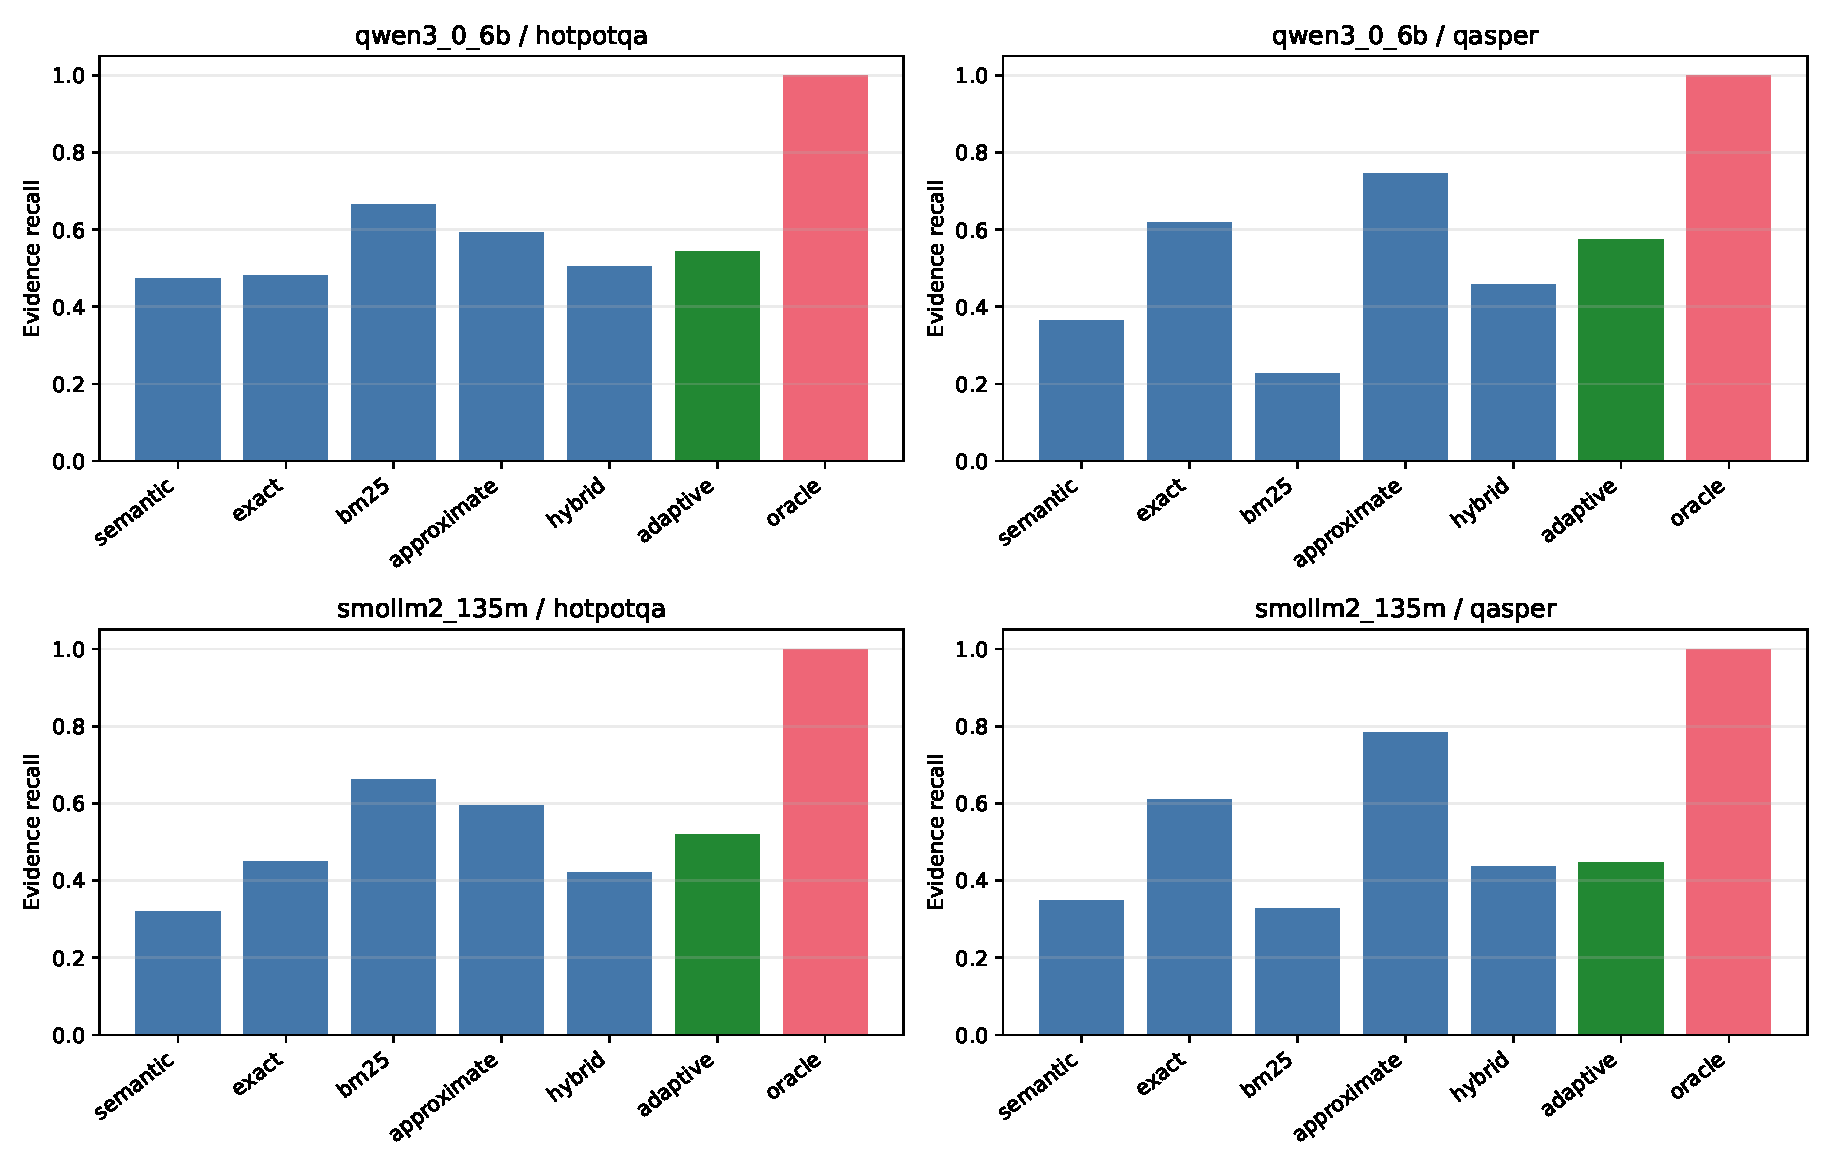
\includegraphics[width=.96\linewidth]{end_to_end_retrieval.pdf}
\caption{Shared-question cross-model evidence recall within the annotation-constructed evaluation. Routed-channel preference follows the dataset more consistently than the model family, while the observable selector stays below the strongest fixed channel. The positional control is reported in Table~\ref{tab:gateb-retrieval}.}
\label{fig:gateb-retrieval}
\end{figure}

\subsection{Routed-Content Likelihood Effects on HotpotQA}
Retrieval becomes useful to PRA only when the frozen model responds beneficially after native-K/V materialization. Gold-answer likelihood is the arithmetic mean of teacher-forced log probabilities over the model tokens of one stored reference continuation. HotpotQA contributes its dataset answer; QASPER contributes the yes/no value from the first eligible annotation. The evaluation does not maximize over additional accepted answers or annotations.

Table~\ref{tab:gateb-consumption} reports paired likelihood effects. On HotpotQA, semantic memory improves mean gold-answer token log probability over disabled PRA by 0.744 for Qwen and 0.185 for SmolLM. For Qwen, the routed semantic payload also beats equal-budget shuffled and irrelevant memory by 0.410 and 0.426, with both intervals excluding zero. Oracle evidence beats equal-budget irrelevant memory by 0.770 and 0.256. These controls establish a content-specific likelihood effect in the stated panels, not a general answer-quality gain.

\begin{table}[H]
\centering
\small
\caption{Held-out consumption effects. Values are paired mean changes in the per-answer-token mean gold log probability with 95\% bootstrap intervals.}
\label{tab:gateb-consumption}
\begin{tabularx}{\linewidth}{llXr}
\toprule
Dataset & Model & Contrast & Effect [95\% CI]\\
\midrule
HotpotQA & Qwen & semantic memory $-$ disabled & $+.744\ [+.414,+1.132]$\\
HotpotQA & Qwen & semantic memory $-$ shuffled & $+.410\ [+.101,+.751]$\\
HotpotQA & Qwen & semantic memory $-$ irrelevant & $+.426\ [+.102,+.803]$\\
HotpotQA & SmolLM & semantic memory $-$ disabled & $+.185\ [+.038,+.345]$\\
HotpotQA & Qwen & oracle evidence $-$ irrelevant memory & $+.770\ [+.508,+1.052]$\\
HotpotQA & SmolLM & oracle evidence $-$ irrelevant memory & $+.256\ [+.163,+.354]$\\
QASPER & Qwen & approximate memory $-$ disabled & $-.013\ [-.190,+.185]$\\
QASPER & SmolLM & approximate memory $-$ disabled & $-.008\ [-.138,+.123]$\\
QASPER & Qwen & oracle evidence $-$ irrelevant memory & $+.154\ [+.074,+.231]$\\
QASPER & SmolLM & oracle evidence $-$ irrelevant memory & $+.091\ [+.033,+.150]$\\
\bottomrule
\end{tabularx}
\end{table}

\subsection{QASPER Separates Retrieval from Consumption}
QASPER approximate matching recovers roughly three quarters of evidence for both models, yet its likelihood change relative to disabled memory is unresolved. The oracle still beats irrelevant memory for Qwen and SmolLM. The materializer and consumer can therefore discriminate maximally correct from wrong memory, but the strongest fixed retriever does not establish a benefit over no memory. In concise form,
\[
\text{retrieval success}\not\Rightarrow\text{useful consumption}.
\]
This counterexample redirects later work toward admission, attention competition, consumer adaptation, and PRA-aware training rather than treating higher recall as sufficient.

Retrieval recall and likelihood also disagree within HotpotQA. For Qwen, BM25 has the highest routed evidence recall (.665) but a smaller disabled-relative likelihood change (+.545) than semantic retrieval (+.744); its shuffled-memory contrast is +.211 with interval $[-.026,+.457]$. The channel that finds more annotated spans is therefore not necessarily the channel whose admitted payload most helps this frozen consumer.

\begin{figure}[H]
\centering
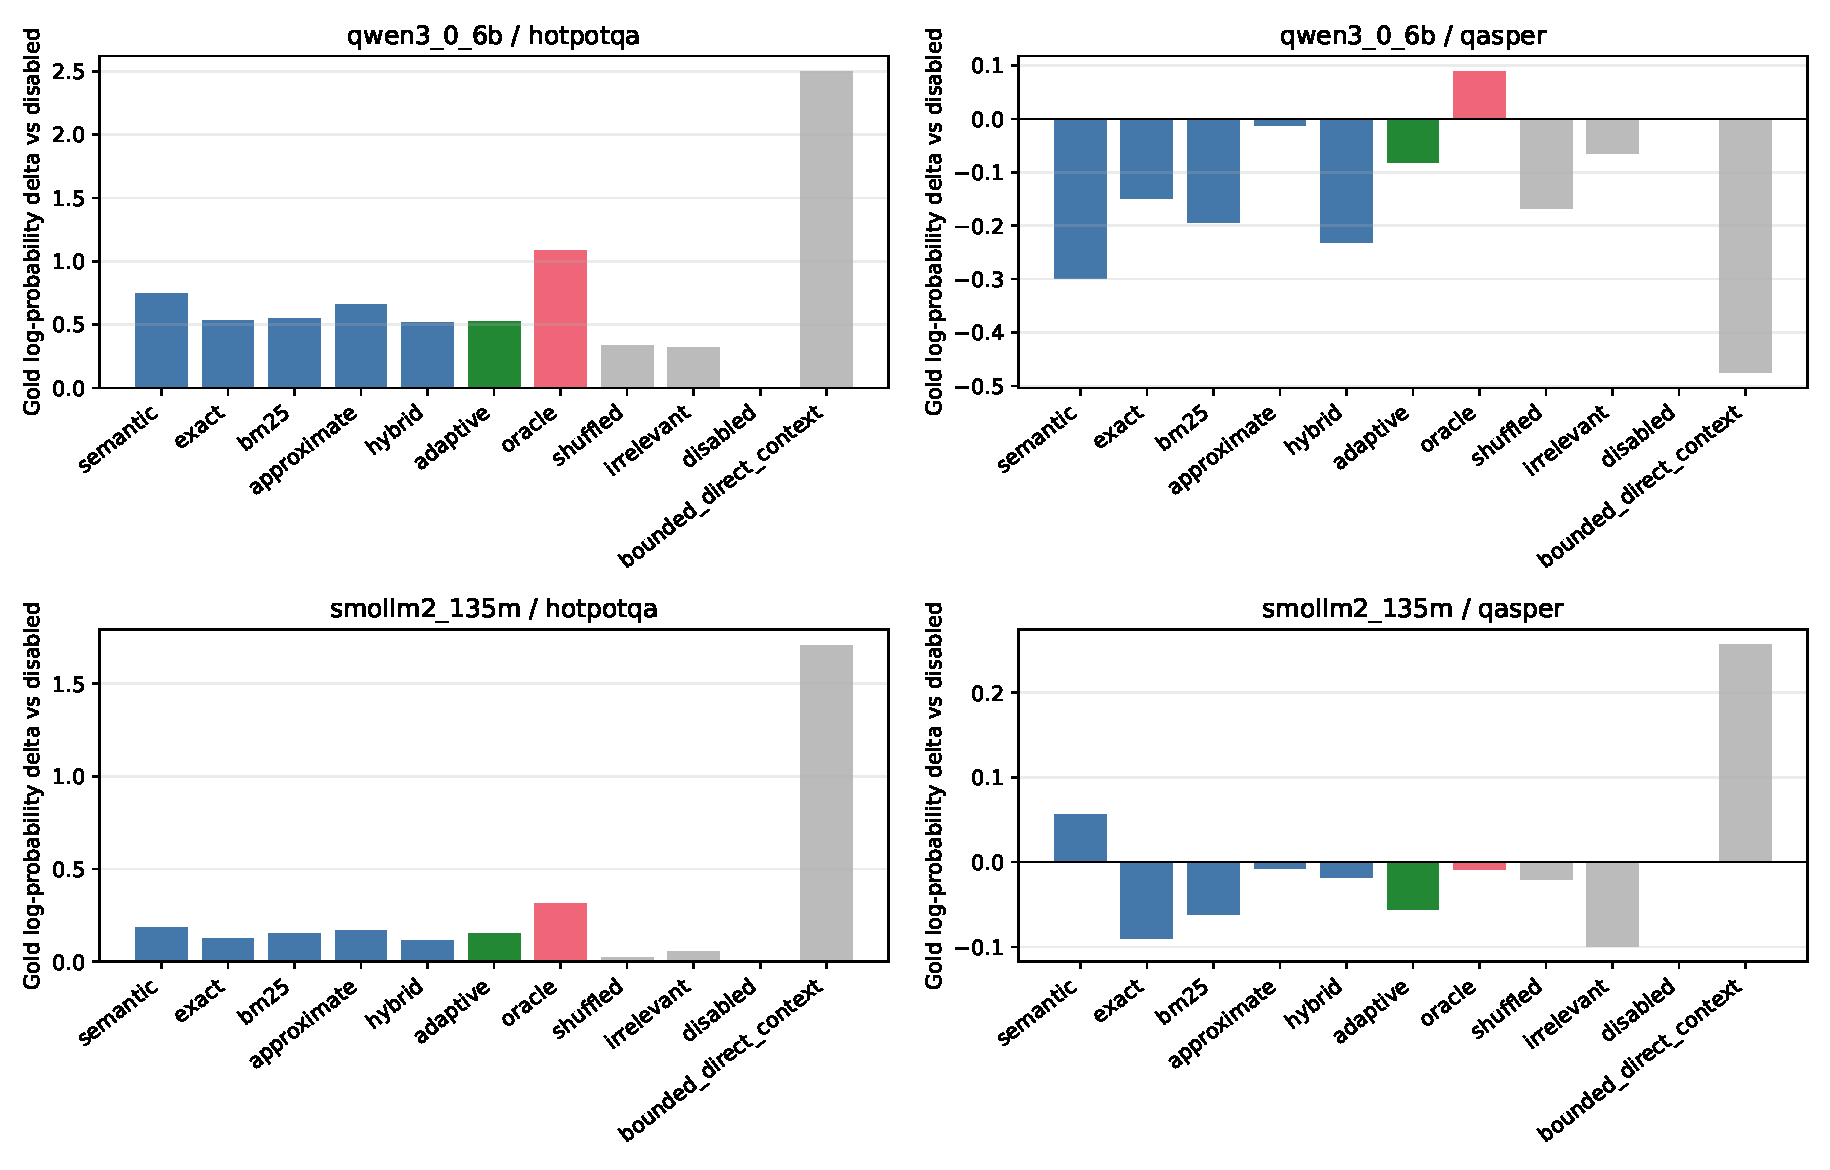
\includegraphics[width=.96\linewidth]{end_to_end_confirmation.pdf}
\caption{Gold-answer likelihood under matched discovery, oracle, wrong-memory, disabled, and bounded direct-context conditions. Direct context is a heavier comparison, not a matched-K/V condition.}
\label{fig:gateb-logp}
\end{figure}

Physical accounting confirms a near match rather than fictitious identity. Mean realized payload ranges from 127.32 to 128.00 unique tokens across routed panels, or 8.33--9.37\% of the bounded source, at each of four late layers. At exactly 128 tokens this is 512 layer-token states. The recorded grouped-query geometries (8 Qwen or 3 SmolLM K/V heads, head width 64, K and V, two bytes per element) imply 1.00~MiB and 0.375~MiB of 16-bit payload. These are formula-derived payload sizes, not allocator measurements. Disabled and empty conditions report zero external PRA K/V; they still use the decoder's ordinary prompt and generation state.

Generated answers remain weak. Qwen semantic-minus-disabled HotpotQA F1 is only $+.00894$ with interval $[-.02971,+.04589]$; it does not establish a generated-answer improvement. Qwen HotpotQA memory conditions obtain EM 0.00--0.02 and F1 0.074--0.120; SmolLM EM is zero. Bounded direct context reaches Qwen HotpotQA F1 0.183 at 5.28~s per example, while 128-token PRA conditions take about 1.4~s at lower quality. These are separate quality--cost operating points, not a quality-matched speedup; source encoding and index construction also have different amortization boundaries. Teacher-forced likelihood is the more sensitive causal endpoint here, and we do not reinterpret it as a QA-accuracy gain.

\section{Breadth: Four-Dataset Channel Geometry}
The held-out mechanism evaluation supplies shared-question model replication and consumption measurements on HotpotQA/QASPER. The earlier frozen-feature cohort adds breadth across QASPER, HotpotQA, 2Wiki, and MuSiQue while holding model, layer, chunk size, and four-chunk request budget fixed. Its QASPER exact winner differs from the approximate winner in the fresh held-out construction; the cohorts and settings differ, so these are not interchangeable estimates. Table~\ref{tab:four-channel} shows a different winning channel on three task regimes. Static and iterative hybrid search improve over semantic gists in several rows but never dominate the best individual channel.

\begin{table}[H]
\centering
\small
\caption{Legacy held-out recall/precision at four requested 32-token chunks. This breadth study is secondary to the fresh held-out mechanism evaluation.}
\label{tab:four-channel}
\resizebox{\linewidth}{!}{%
\begin{tabular}{lrrrrrr}
\toprule
Dataset ($n$) & Gist & Exact & BM25 & Approx. & Static hybrid & Iterative hybrid\\
\midrule
QASPER (16) & .038/.062 & \textbf{.178}/.312 & .042/.094 & .037/.078 & .044/.078 & .081/.125\\
HotpotQA (16) & .151/.172 & .287/.328 & \textbf{.398}/.453 & .301/.359 & .288/.344 & .279/.312\\
2Wiki (24) & .132/.188 & .196/.240 & \textbf{.262}/.312 & .203/.250 & .203/.250 & .186/.250\\
MuSiQue (18) & .108/.333 & .136/.417 & .132/.431 & \textbf{.156}/.514 & .151/.500 & .146/.472\\
\bottomrule
\end{tabular}}
\end{table}

\begin{figure}[H]
\centering
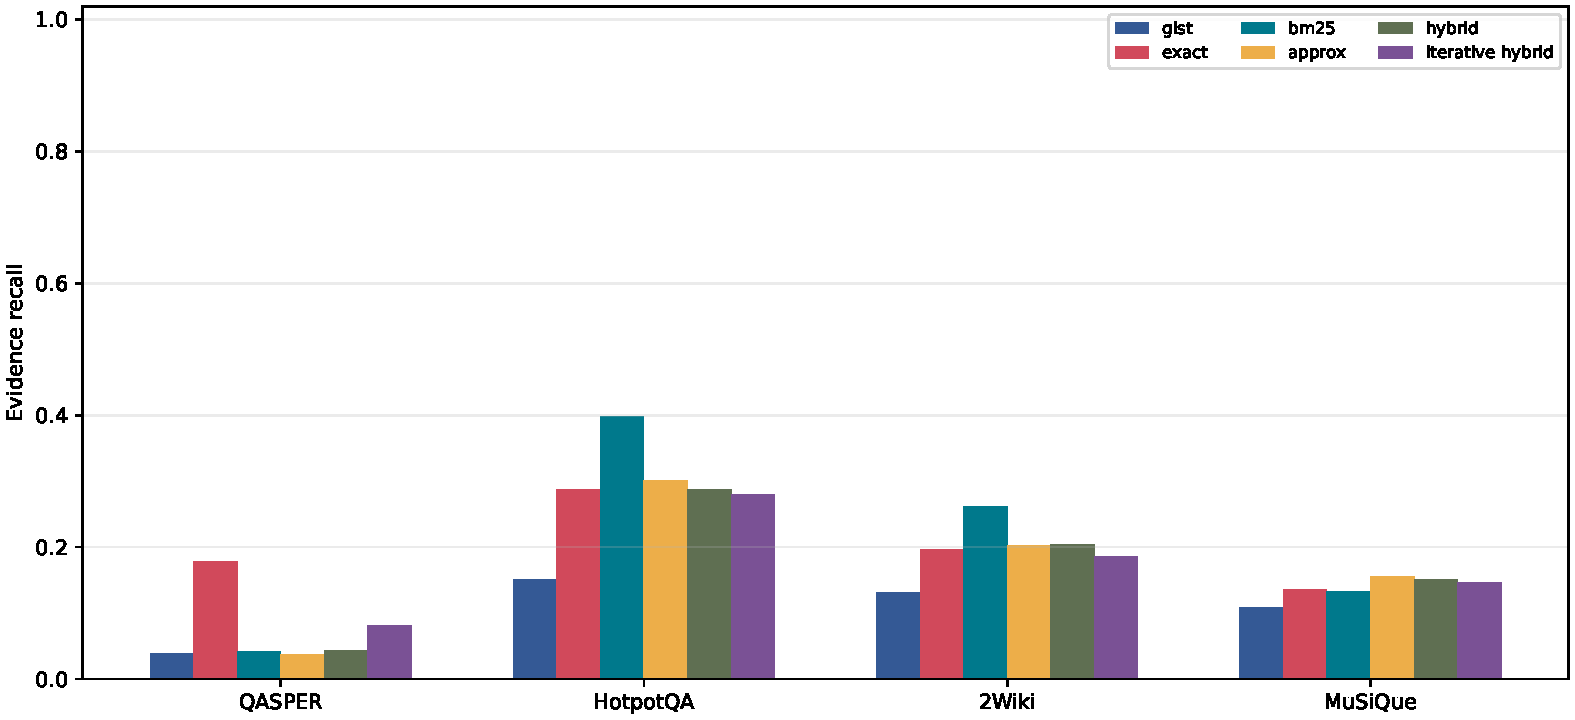
\includegraphics[width=.96\linewidth]{channel_recall.pdf}
\caption{Matched-budget recall in the four-dataset breadth cohort. No representation dominates all cohorts, and static fusion does not reliably beat the strongest individual channel.}
\label{fig:channel-breadth}
\end{figure}

The representations are genuinely nonredundant. Mean selected-set Jaccard across channel pairs is 0.256 on QASPER, 0.325 on HotpotQA, 0.369 on 2Wiki, and 0.326 on MuSiQue. Yet complementarity alone does not make fusion better: at a two-chunk root budget, lexical channels add 0.188--0.812 unique gold chunks per example relative to gist search while adding 2.778--3.500 unique distractors. Reciprocal-rank fusion avoids raw-score calibration but also fails to dominate. Meaning and identity are complementary signals; their distractors are complementary too.

\section{Root and Successor Search Are Different Decisions}
We next divide the four-chunk budget into two root and two successor chunks. Every root representation is crossed with every successor representation, but the successor headline fixes the root policy selected on validation. For 2Wiki and MuSiQue, successor truth follows annotated dependency nodes. QASPER and HotpotQA provide unordered evidence remainders, so their successor rows diagnose staged retrieval without asserting a gold dependency edge.

\begin{table}[H]
\centering
\small
\caption{Best held-out root and successor representations under the validation-selected root. R/P are stage-local evidence recall and precision.}
\label{tab:root-successor}
\begin{tabularx}{\linewidth}{lXrXr}
\toprule
Dataset & Root representation & Root R/P & Successor representation & Successor R/P\\
\midrule
QASPER & exact & .096/.312 & exact new address & .025/.125\\
HotpotQA & exact & .047/.094 & native semantic & .135/.281\\
2Wiki & semantic gist & .076/.125 & exact new address & .050/.083\\
MuSiQue & approximate & .084/.139 & native semantic & .032/.111\\
\bottomrule
\end{tabularx}
\end{table}

\begin{figure}[H]
\centering
\begin{minipage}{.49\linewidth}\centering
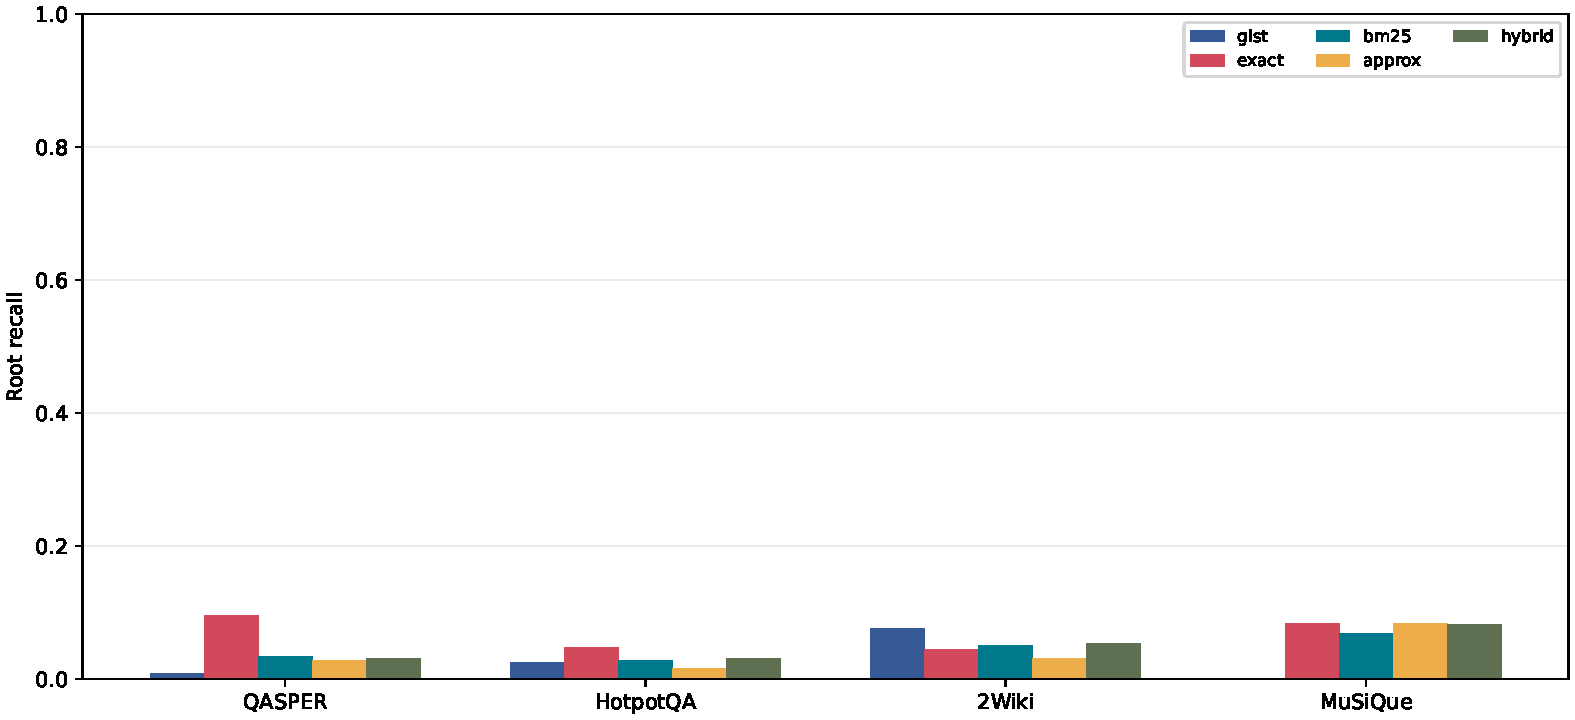
\includegraphics[width=\linewidth]{root_recall.pdf}
\end{minipage}\hfill
\begin{minipage}{.49\linewidth}\centering
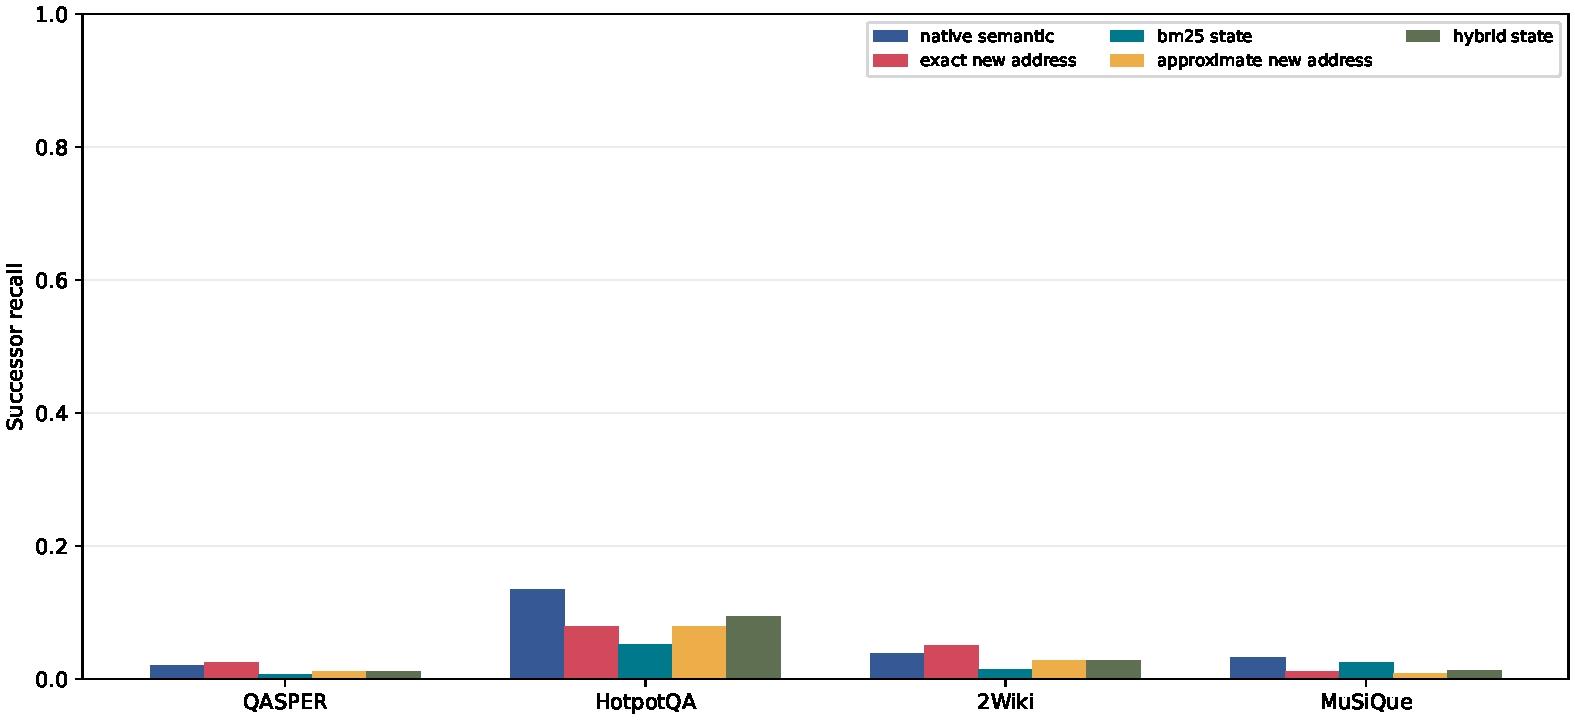
\includegraphics[width=\linewidth]{successor_recall.pdf}
\end{minipage}
\caption{Root recall at two chunks and successor recall at two chunks under a fixed root policy. The preferred representation changes after admission on three of four datasets.}
\label{fig:root-successor}
\end{figure}

QASPER retains exact identity at both stages. HotpotQA and MuSiQue prefer lexical root entry but semantic successor expansion. 2Wiki prefers semantic entry and an exact newly exposed address. No per-example oracle transition occupies a majority. These low absolute recalls do not show that the staged router solves multi-hop retrieval; they show that forcing root and successor through one score discards a measurable action dimension.

Simple observable selectors do not recover the oracle. A validation-trained linear selector remains below the best held-out fixed channel on three datasets and ties only MuSiQue. Root disagreement has correlation 0.052 with true per-example oracle headroom. Paper~2.6 therefore exports $S_{\mathrm{root}}$ and $S_{\mathrm{succ}}$ as actions rather than claiming adaptive control. Full oracle, selector, confidence, and transition diagnostics appear in Appendices~\ref{app:selector} and~\ref{app:root-successor}.

\section{Representation, Budget, Granularity, and Model}
The interaction study crosses eight channels with 16-, 32-, and 64-token chunks, Top-2/4/8 selection, early/late routing layers, two datasets, and two model families. Its eight examples per dataset are disjoint from the legacy, validation, and held-out test sets. Because it contains only 16 identities, it diagnoses coupling rather than replacing the held-out evaluation.

At 32-token granularity, broader selection buys coverage at the cost of selectivity. Averaged over channels, late-layer Qwen HotpotQA recall rises from 0.562 to 0.703 to 0.883 as Top-$K$ grows from 2 to 4 to 8; complete recovery rises from 0.406 to 0.562 to 0.812, while precision falls from 0.414 to 0.229. SmolLM follows the same pattern, reaching 0.953 recall and 0.906 complete recovery at Top-8 while precision falls to 0.225. QASPER reaches 0.917 and 0.943 recall at Top-8 for Qwen and SmolLM. Thus
\[
\boxed{\text{breadth buys coverage at the cost of selectivity}}.
\]

\begin{figure}[H]
\centering
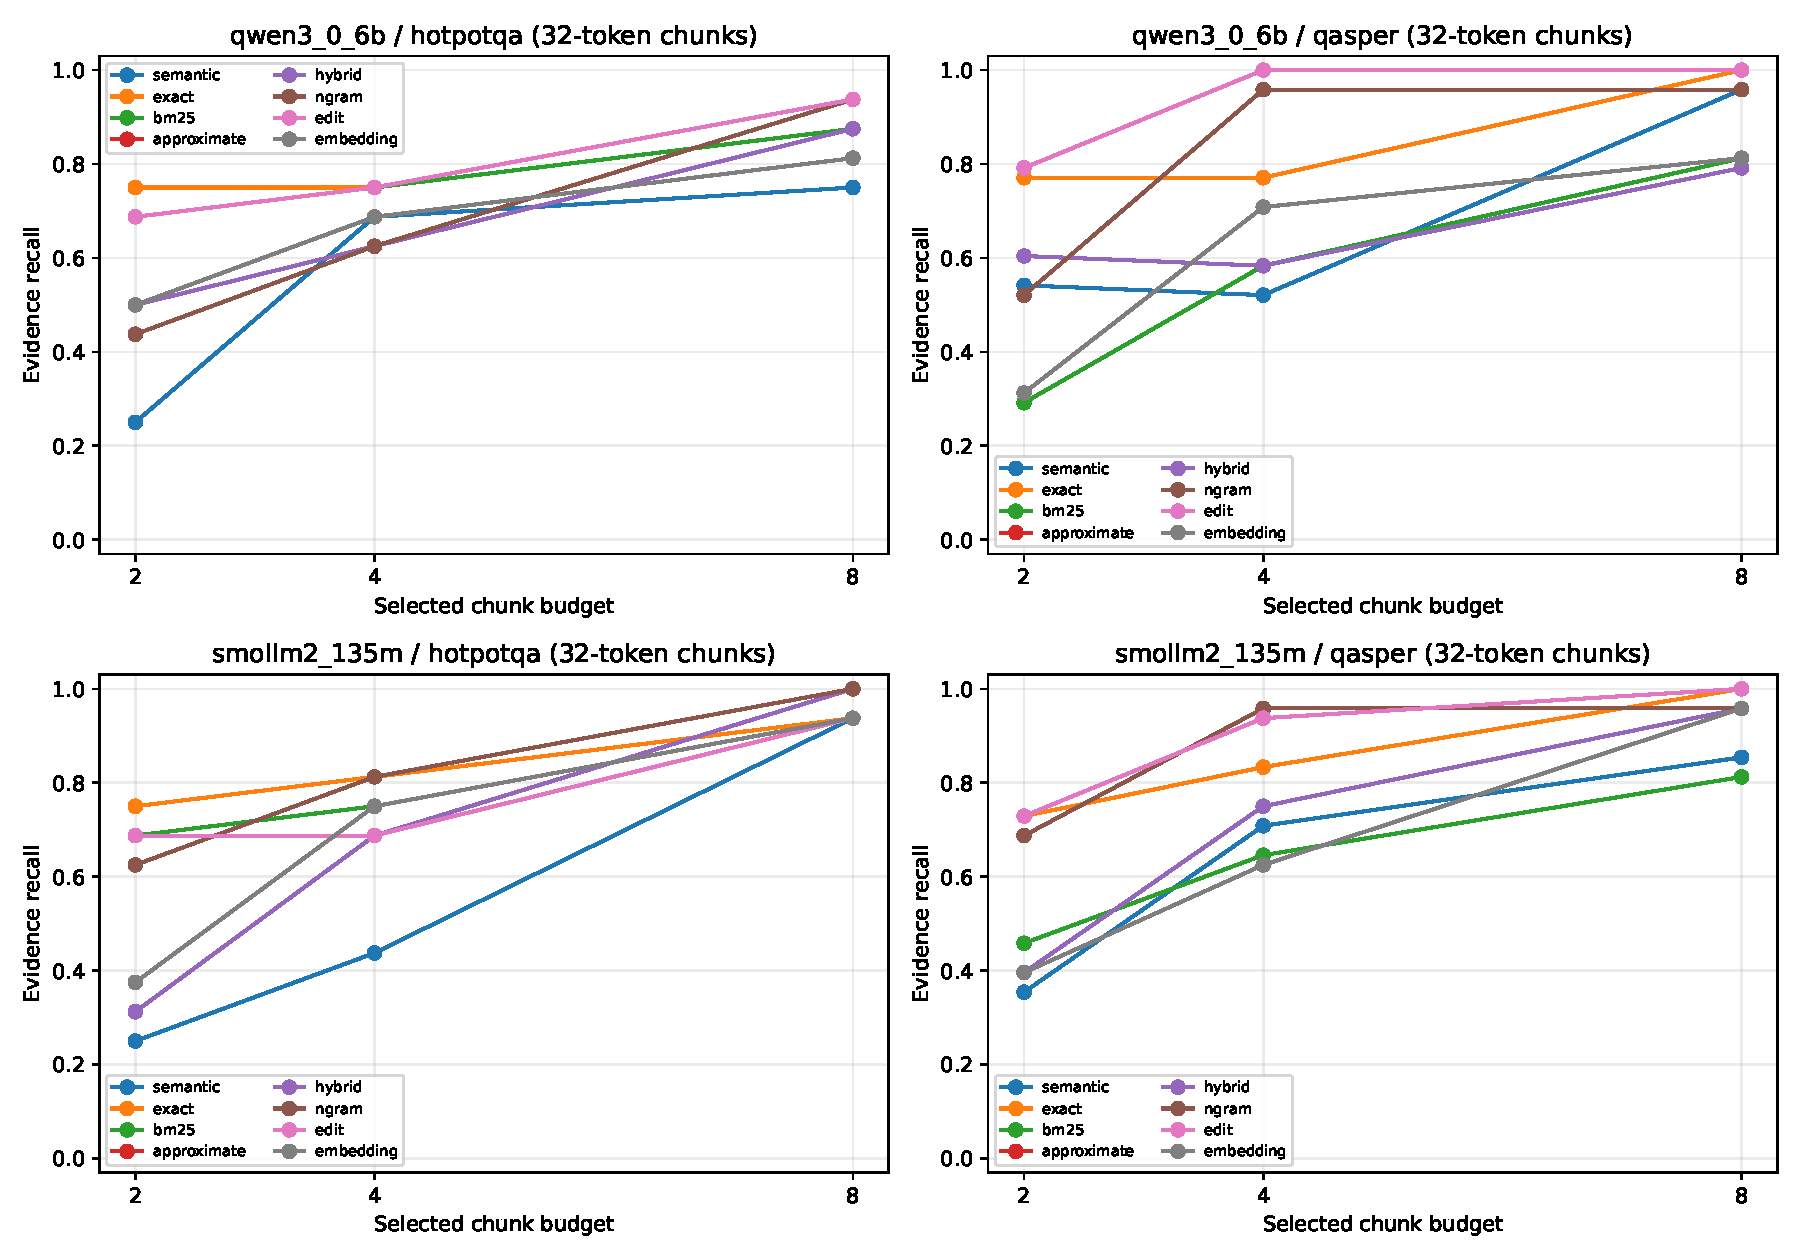
\includegraphics[width=.96\linewidth]{hybrid_budget_interactions.pdf}
\caption{Evidence recall as the reachable selected-chunk budget grows at fixed 32-token granularity. Additional chunks recover more evidence and admit more distractors.}
\label{fig:budget}
\end{figure}

Holding routed physical tokens fixed at 128 reveals a second interaction. The best channel changes with chunk size, dataset, and model. Qwen/HotpotQA favors token $n$-grams at 16 and 64 tokens but bounded edit at 32; SmolLM/QASPER favors hybrid at 16, token $n$-grams at 32, and exact at 64. Token-native channels are layer invariant by construction, but semantic recall changes between measured early and late layers by $+0.174$, $+0.046$, $+0.021$, and $-0.039$ across the four model/dataset pairs. Late hidden states are not automatically better routing representations.

The secondary relationship is therefore
\[
S^*=f(\text{task},\text{model},\text{granularity},\text{budget},\text{stage})
\]
within the measured scope. This is a reason to expose configuration dimensions, not evidence for a universally optimal setting. Detailed matched-token rows and the reachability audit appear in Appendix~\ref{app:interactions}.

\section{Discussion}
\paragraph{Meaning and identity are complementary.}
Semantic gists recover contextual relations, while exact, BM25, and approximate channels preserve different surface evidence. Repeated ordering across two tokenizers/models on the same held-out questions makes this more than a one-tokenizer curiosity, but it is not independent task-sample replication and all primary sources are annotation constructed.

\paragraph{Static fusion is not enough.}
Channels retrieve complementary evidence and complementary distractors. Under a small working-set budget, uncalibrated union or rank fusion can spend scarce slots on the latter. The useful object is an explicit retrieval action with provenance, not a larger undifferentiated score vector.

\paragraph{Sparse discovery is feasible, but the fuzzy path is unfinished.}
Posting lists preserve the measured Top-4 outputs on synthetic templated queries while reducing final scoring work and exact-query latency relative to exhaustive Python. The semantic reserve still needs full-corpus scores and sorting. Character and edit-based fallback consumes hundreds of milliseconds, and the current immutable rebuild is not an incremental production index.

\paragraph{Retrieval and consumption are distinct bottlenecks.}
HotpotQA supplies the positive bridge: routed semantic memory changes frozen-model likelihood relative to disabled and wrong-memory controls, while generated F1 remains unresolved. QASPER supplies the limiting case: high retrieval recall does not establish a fixed-channel gain over disabled memory. Later PRA work must study admission, attention competition, model adaptation, and training alongside retrieval.

\paragraph{Representation belongs in the control interface.}
Root and successor choices differ, and channel preference interacts with granularity and budget. The versioned action contract preserves independent root/successor methods, confidence status, provenance, and cost fields for adaptive control in Paper~3.5~\cite{simao2026adaptive}. Paper~3 separately controls how selected identities become physical K/V~\cite{simao2026materialization}.

\section{Related Work}
\paragraph{Sparse, dense, and hybrid retrieval.}
BM25 and dense passage retrieval represent established lexical and semantic retrieval families~\cite{robertson2009bm25,karpukhin2020dpr}. RAG supplies retrieved text to a generator, while reciprocal-rank fusion combines ranked lists without assuming comparable score scales~\cite{lewis2020rag,cormack2009rrf}. Hybrid IR is not our novelty. We study how these representation families address stable PRA memory identities under a native-K/V working-set budget, and we retain the negative result that static fusion need not beat its strongest component.

\paragraph{Multi-hop retrieval.}
MDR conditions later dense retrieval on earlier passages; IRRR builds a reasoning path, forms a next search query, reranks, and decides whether to continue; IRCoT interleaves retrieval with generated reasoning~\cite{xiong2021mdr,qi2021irrr,trivedi2023ircot}. PRA similarly changes state after admission, but its search operates over identities aligned to reusable native-memory objects. Our narrower result is that the representation itself can change between root and successor stages.

\paragraph{Reference resolution.}
Approximate matching handles insertions, deletions, substitutions, and related surface changes~\cite{navarro2001approx}. Contextual entity linking, such as BLINK's bi-encoder retrieval and cross-encoder reranking, addresses the harder problem of resolving ambiguous mentions~\cite{wu2020blink}. Our token-native resolver is intentionally lighter. Its typo and alias gains coexist with stale-alias and wrong-instance failures, so it should not be read as a full entity linker.

\paragraph{Long-context and K/V memory.}
RETRO retrieves neighboring text chunks into a trained decoder, while Memorizing Transformers query a store of prior activation keys and values~\cite{borgeaud2022retro,wu2022memorizing}. Quest and RetrievalAttention perform query-aware physical K/V selection or indexing~\cite{tang2024quest,liu2025retrievalattention}. Paper~2.6 operates primarily upstream, discovering identity-bearing logical objects, then uses the held-out mechanism evaluation to test their native-K/V consumption. The distinction is
\[
\boxed{\text{logical memory discovery}}\neq
\boxed{\text{physical K/V selection or compression}}.
\]

\section{Limitations}
The primary evaluation covers two small frozen model families and only HotpotQA/QASPER. Both models reuse the same held-out identities. Its evidence-first bounded construction is annotation dependent, nearly saturates a first-four positional baseline, and frequently duplicates evidence in the appended source; it does not reproduce an unmodified document benchmark. Original-order, randomized-location, and fully deduplicated-source conditions are unperformed, so claims are restricted to mechanism behavior under the constructed source. 2Wiki and MuSiQue appear only in the smaller legacy frozen-feature breadth study. The interaction cohort has eight examples per dataset. Five selector seeds measure optimization variability, not independent sample uncertainty.

Generated EM/F1 is weak, and the positive end-to-end claim is limited to paired gold-answer likelihood on HotpotQA. The likelihood metric scores one stored continuation and does not maximize over multiple acceptable answers. QASPER fixed-channel consumption remains unresolved. Natural top-reference correctness is only an evidence-overlap proxy, not adjudicated coreference. Validation-fitted confidence does not transfer reliably, confidently wrong references remain possible, and the tested learned ensemble does not close the fixed-channel gap.

The index study uses synthetic rows and templated queries. Its candidate fraction excludes semantic-score production, and its payload estimate excludes Python-object memory. It rebuilds corpus statistics on update. Exact lookup is promising, but 0.50--0.65~s fuzzy routes are not production ready. The study does not compare an optimized production lexical engine or test arbitrary-query parity, larger models, learned contextual entity linking, incremental serving indexes, larger selector-training sets, or PRA-aware fine-tuning. Failure to reproduce measured-suite indexed parity, shared-question channel ordering, or the paired routed-content effects would falsify the corresponding claims independently.

\section{Conclusion}
Within the annotation-constructed sources, semantic meaning, exact identity, BM25-weighted terms, and approximate surface matching recover different evidence, and their dataset-level preferences repeat across two tested model/tokenizer families on shared questions. Yet the near-saturating positional control prevents interpreting these results as an ordinary retrieval benchmark, and the tested adaptive ensemble does not beat its fixed comparator. Sparse posting-list narrowing preserves measured synthetic-suite Top-4 behavior while reducing prototype work relative to exhaustive Python. Routed HotpotQA semantic memory then produces a content-specific frozen-model likelihood effect after native-K/V admission, without a resolved generated-F1 gain.

The boundary is equally important. QASPER shows that high evidence recall does not guarantee useful fixed-channel consumption. Root and successor search can prefer different representations descriptively, static fusion does not reliably solve that heterogeneity, and simple observable selectors remain inadequate. Paper~2.6 therefore solves neither general document retrieval, adaptive control, nor consumer training. It supplies a measured multi-representational discovery interface and identifies where retrieval-to-consumption remains open.

\appendix
\section{Original Discovery Experiment}
\label{app:original}
The original Qwen frozen-feature experiment used eight validation and 16 held-out examples per dataset, layer-27 attention-input states, 32-token mean gists, and four requested chunks. It predates the fresh held-out campaign and is retained for provenance rather than treated as primary evidence. Broad semantic Top-8 deliberately used twice the request budget; the oracle admitted annotated evidence and is only a ceiling.

\begin{table}[H]
\centering
\scriptsize
\caption{Original held-out discovery. R/P/M are supporting-evidence recall, precision, and MRR. B0--H5 request four chunks; A1 requests eight.}
\resizebox{\linewidth}{!}{%
\begin{tabular}{lrrrrrr}
\toprule
& \multicolumn{3}{c}{HotpotQA} & \multicolumn{3}{c}{QASPER}\\
Condition & R & P & M & R & P & M\\
\midrule
gist & .151 & .172 & .276 & .038 & .062 & .130\\
BM25 & .398 & .453 & .875 & .042 & .094 & .135\\
exact & .287 & .328 & .568 & .178 & .312 & .443\\
weighted & .287 & .328 & .568 & .061 & .109 & .214\\
approximate & .301 & .359 & .734 & .037 & .078 & .141\\
union & .209 & .250 & .365 & .038 & .062 & .130\\
token$\rightarrow$semantic & .287 & .344 & .635 & .044 & .078 & .125\\
semantic$\rightarrow$token & .279 & .328 & .635 & .052 & .094 & .156\\
cascade & .240 & .281 & .474 & .126 & .203 & .307\\
iterative hybrid & .279 & .312 & .646 & .081 & .125 & .177\\
broad semantic & .310 & .180 & .363 & .088 & .078 & .155\\
oracle & .876 & 1.000 & 1.000 & .633 & 1.000 & 1.000\\
\bottomrule
\end{tabular}}
\end{table}

Iterative hybrid improves HotpotQA gist recall by 0.129, with paired 95\% bootstrap interval $[0.018,0.242]$, but remains below BM25. Its QASPER improvement over gist is 0.043 with interval $[-0.014,0.111]$; exact instead improves by 0.140 with interval $[0.053,0.244]$. These small-cohort results anticipated representation heterogeneity but are superseded by the fresh held-out evaluation for HotpotQA/QASPER.

\section{Full Four-Dataset Geometry}
\label{app:geometry}
Best-channel paired intervals in the breadth cohort are QASPER $[.096,.271]$, HotpotQA $[.282,.516]$, 2Wiki $[.176,.353]$, and MuSiQue $[.122,.194]$. High IDF-weighted query/evidence overlap is associated with a 0.200 best-lexical-over-gist advantage, compared with 0.131 below the median. Examples with at least the median three distinct root choices have mean lexical advantage 0.197, versus 0.101 below the median. These are gold-derived explanatory strata, not deployable selector inputs.

\begin{figure}[H]
\centering
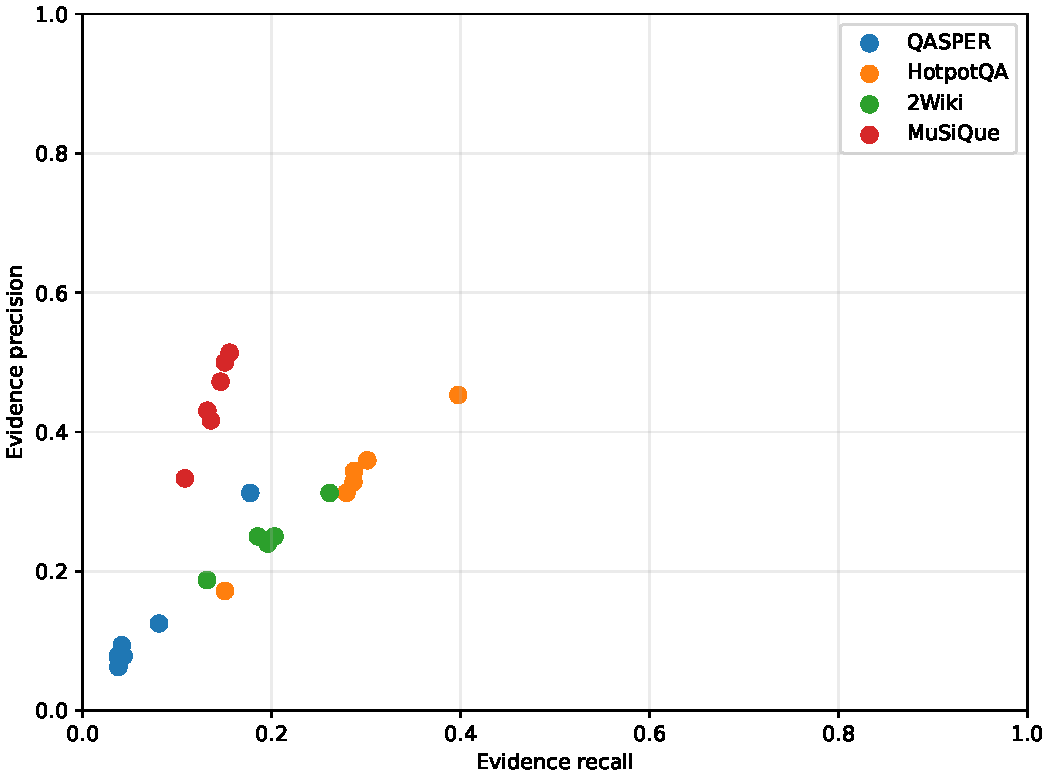
\includegraphics[width=.72\linewidth]{channel_precision_recall.pdf}
\caption{Full precision--recall surface for the four-dataset breadth cohort. Improved recall through union is not automatically a better policy when precision falls.}
\end{figure}

The per-example four-chunk oracle reaches recall 0.207, 0.489, 0.315, and 0.199 on QASPER, HotpotQA, 2Wiki, and MuSiQue. Earlier ``headroom'' values mixed true adaptive opportunity with validation-selected channel reversal; Appendix~\ref{app:selector} gives the corrected decomposition. Full per-example rows, pairwise Jaccard matrices, lexical strata, and disagreement diagnostics are committed under \path{channel_geometry/}.

\section{Selectors, Confidence, and Referential Validity}
\label{app:selector}
At the two-chunk root stage, true per-example selection headroom $H_{selection}$ is 0.014, 0.021, 0.053, and 0.013 across QASPER, HotpotQA, 2Wiki, and MuSiQue. Validation instability $H_{validation}$ is 0, 0.031, 0.026, and 0. The corresponding successor values are $0.027/0$, $0.028/0.056$, $0.056/0.011$, and $0.016/0.008$. Only the 2Wiki root and MuSiQue successor paired intervals exclude zero. The action opportunity is real but small calibration splits cannot choose it reliably.

The leakage-audited replay exports 1,255 candidate rows with top score, score gap, entropy, support, span length, rarity, ambiguity, cross-channel agreement, semantic consistency, path consistency, and source consistency. Dataset identity, answer text, evidence geometry, and oracle labels are forbidden inputs. Validation-CDF confidence is poorly calibrated: mean root AUROC is 0.424, mean successor AUROC 0.526, and mean ECE 0.401 and 0.456. A semantic consistency gate never improves root top-one correctness over lexical confidence. The observable UsefulAddress proxy reaches AUROC 0.555 and AUPRC 0.230 over 68 successor-bearing identities.

\begin{figure}[H]
\centering
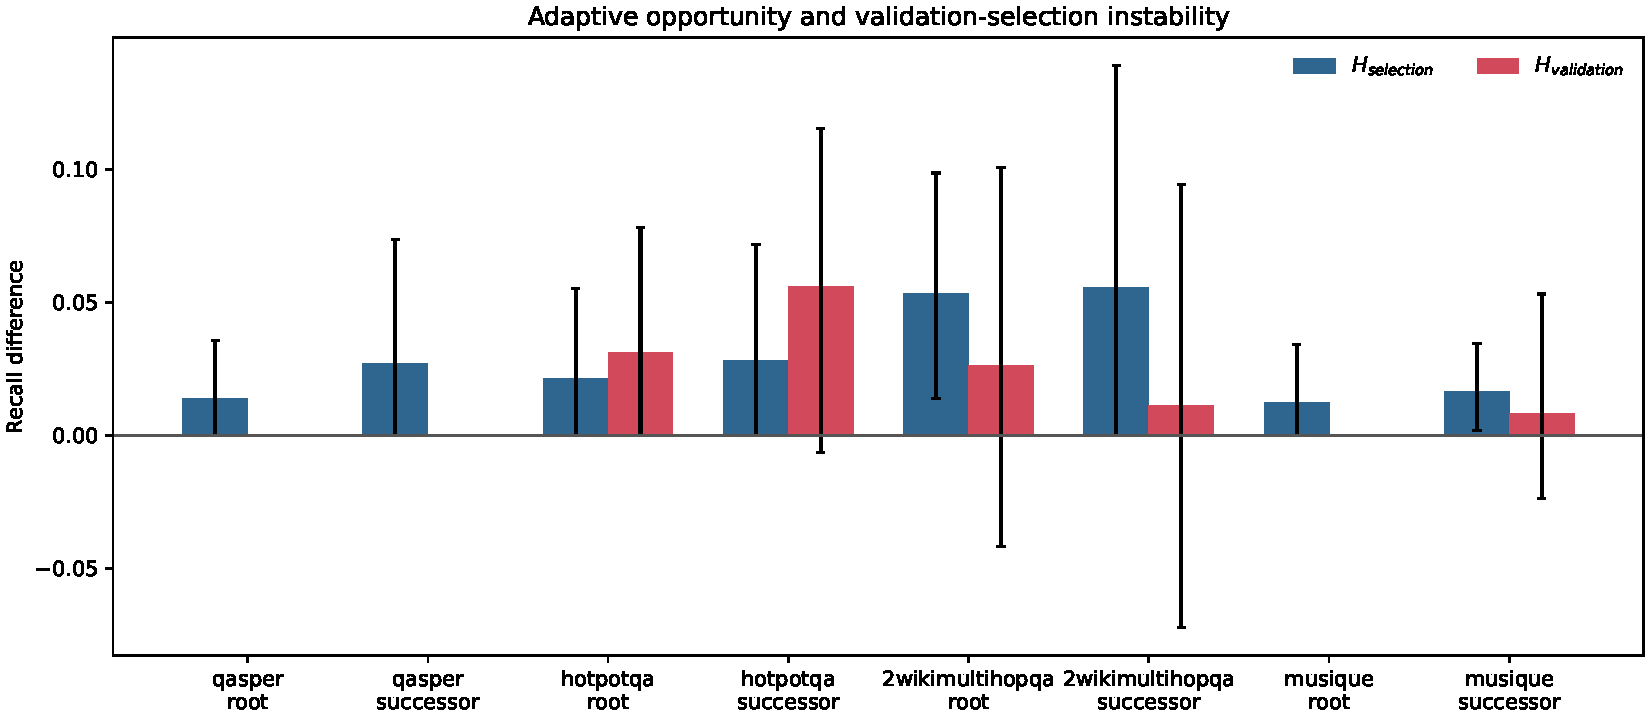
\includegraphics[width=.94\linewidth]{adaptive_headroom_updated_ci.pdf}
\caption{True selection opportunity and validation instability with identity-paired bootstrap intervals. Oracle effects remain diagnostic ceilings.}
\end{figure}

Natural held-out top-reference accuracy further shows that retrieval score is not referential probability. Approximate top-one accuracy is 0.94 on HotpotQA but only 0.36--0.40 on QASPER. Except for approximate HotpotQA, validation thresholds targeting 0.80 precision transfer below 0.64 and often below 0.20 held-out precision.

\section{New Addresses and Controlled Chains}
\label{app:addresses}
A strict new address is absent from the question, present in an admitted root and unrecovered gold evidence, and rare under local IDF. Such addresses appear in 6/16 QASPER, 5/16 HotpotQA, 10/24 2Wiki, and 15/18 MuSiQue examples. Exposure alone does not predict iterative gain. The stricter UsefulAddress predicate additionally requires a gold-linked successor to rank within four; it predicts positive hybrid-state gain only in the measured MuSiQue subset.

Twenty deterministic trials per condition test clean, case, punctuation, typo, alias, and conflicting-reference chains. Iterative hybrid recovers every clean, case, and punctuation target, half of typo targets, and none when the exposed address confidently names the wrong object. Exact search fails on typos; approximate search repairs every typo and half of alias cases, but follows stale aliases and wrong instances. These fixtures demonstrate mechanism and failure modes, not natural-frequency estimates.

\begin{figure}[H]
\centering
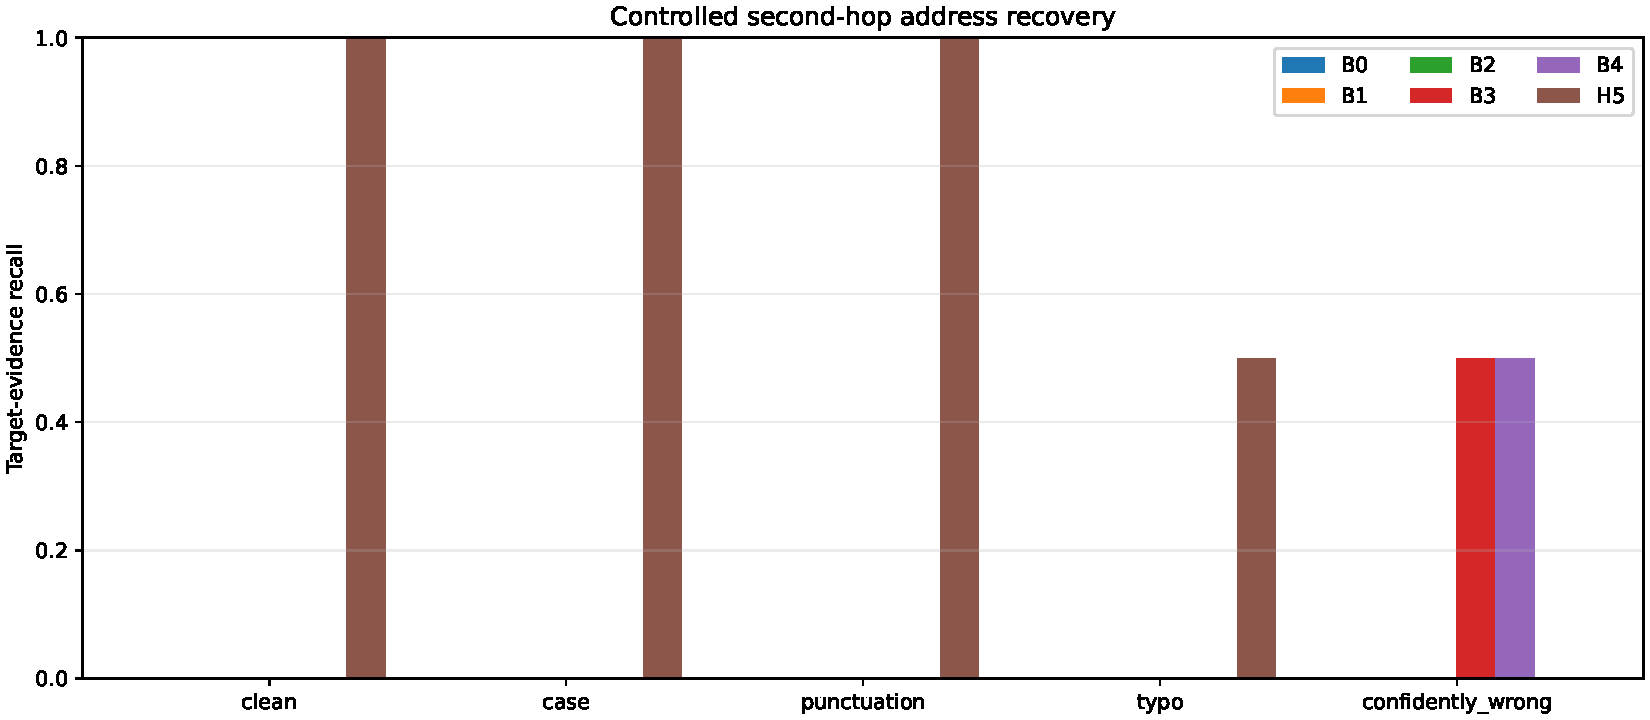
\includegraphics[width=.92\linewidth]{synthetic_perturbations.pdf}
\caption{Controlled second-hop recovery. A newly exposed address can enable retrieval, but confidently wrong references produce catastrophic failure.}
\end{figure}

\section{Tokenizer and Surface-Form Robustness}
\label{app:tokenizer}
The expanded suite covers case, punctuation, leading-space artifacts, whitespace splitting, hyphenation, concatenation, misspellings, abbreviations, aliases, Unicode compatibility forms, near entities, shared prefixes, identifiers, URLs, same-name and same-class ambiguity, wrong relations, stale aliases, and contradictory high-overlap names. Across 13 primary perturbations, cascade recall@4 is 0.985 with corpus IDF and 0.969 with no suppression or a fixed stop list, identically for Qwen and SmolLM tokenizers. Exact reaches 0.923, token $n$-grams 0.754, approximate 0.262, and bounded edit 0.246.

\begin{figure}[H]
\centering
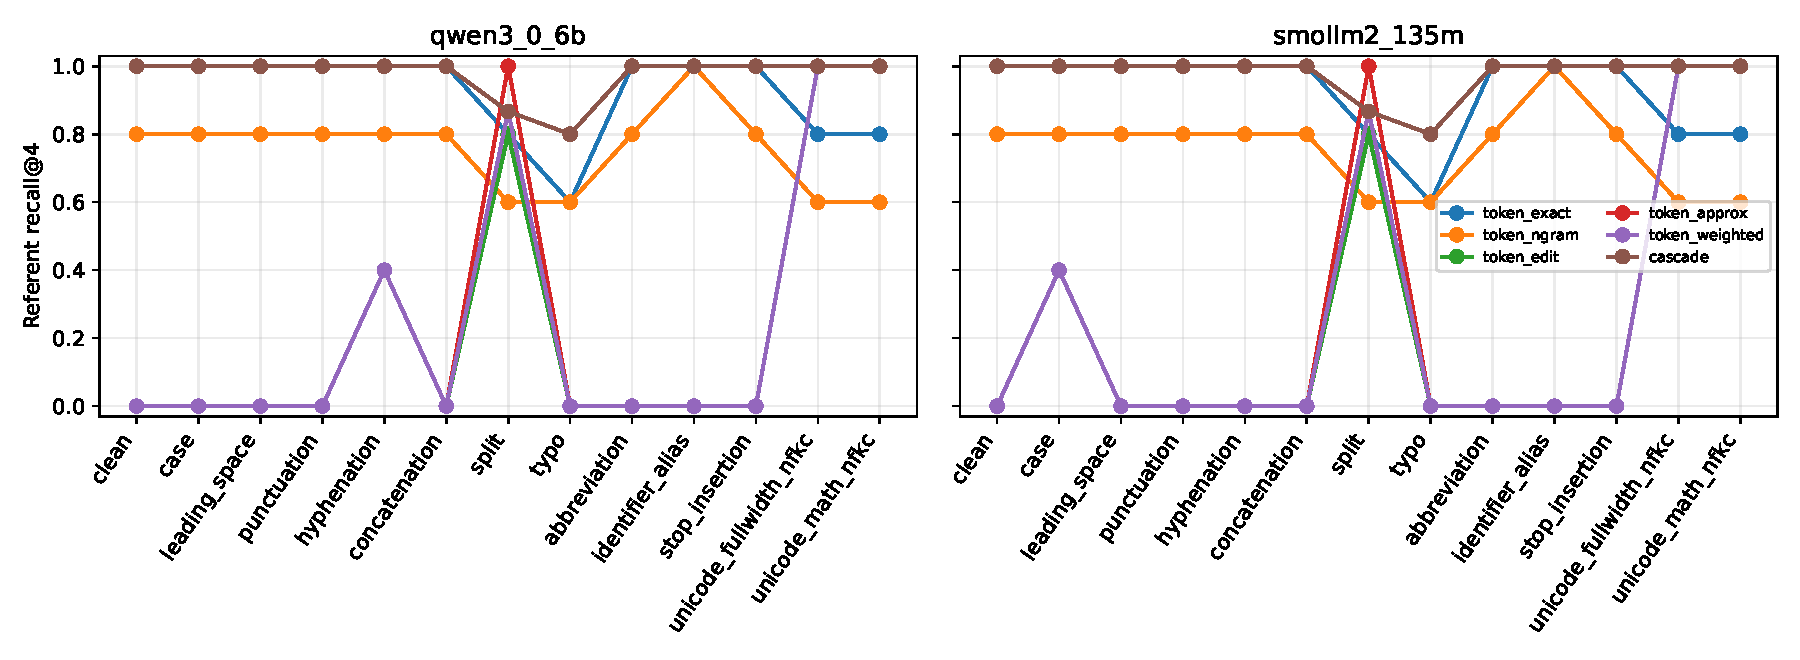
\includegraphics[width=.88\linewidth]{tokenizer_invariance.pdf}
\caption{Controlled target recovery across tokenizers and perturbations. NFKC handles compatibility forms; fallback stages cover some genuinely changed sequences.}
\end{figure}

\section{Wrong-Reference Fixtures}
\label{app:wrong-reference}
The controlled suite includes stale aliases, wrong instances, wrong relations, same-name collisions, contradictory high-overlap references, and two plausible references. Stale aliases route to the wrong target in every exact, approximate, and hybrid trial. Approximate search selects the same-class wrong instance in every trial; exact and hybrid do so in half. Under a correct-entity/wrong-relation fixture, approximate search splits between valid and wrong targets while exact and hybrid recover neither. Threshold rejection creates a fixture-specific abstention opportunity, but no threshold is deployment calibrated.

\begin{figure}[H]
\centering
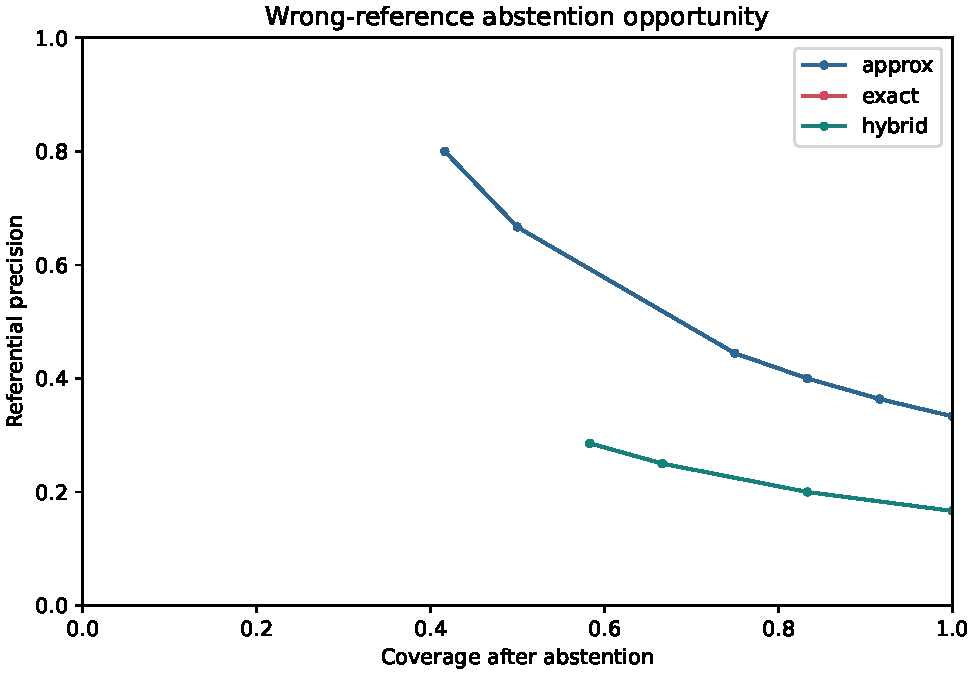
\includegraphics[width=.72\linewidth]{wrong_reference_abstention_precision_recall.pdf}
\caption{Controlled referential precision against retained coverage. This is an abstention opportunity bound, not a natural policy result.}
\end{figure}

\section{Indexed Implementation and Cost}
\label{app:index}
\begin{table}[H]
\centering
\small
\caption{Warm routing at 4,096 synthetic chunks with templated identifier queries. Milliseconds are per query against the matching exhaustive Python implementation; payload MiB excludes Python-object overhead and model inference.}
\begin{tabular}{llrrrr}
\toprule
Tokenizer & Channel & Exhaustive & Indexed & Speedup & Payload MiB\\
\midrule
Qwen & exact & 33557 & 119 & 283x & 10.06\\
Qwen & weighted & 31375 & 530 & 59x & 10.06\\
Qwen & approximate & 31141 & 499 & 62x & 10.06\\
Qwen & cascade & 30965 & 556 & 56x & 10.06\\
SmolLM & exact & 37048 & 125 & 300x & 10.94\\
SmolLM & weighted & 37440 & 649 & 58x & 10.94\\
SmolLM & approximate & 37005 & 632 & 59x & 10.94\\
SmolLM & cascade & 36886 & 577 & 64x & 10.94\\
\bottomrule
\end{tabular}
\end{table}

\texttt{TokenNativeIndex} in \path{src/pra_hf/hybrid_discovery.py} owns aligned rows, tokenization, postings, aliases, payload estimates, immutable rebuilds, and channel scoring. Its candidate-union method ranks at most half of the 64-row pool from lexical posting votes, fills the remainder from a full semantic-score ranking, inserts explicit URI rows, and deduplicates stable identities. Thus the final scorer is sparse while semantic candidate production is not yet sparse. Expensive final-scoring feature families are gated by the requested channel. \texttt{IterativeGistRouter.route} in \path{src/pra_hf/iterative.py} performs root and successor sparse scoring, scatters returned rows into the aligned tensor index, and reuses the inherited visited-set, branch, beam, depth, confidence, and unique-chunk limits.

\texttt{PRAForCausalLM} constructs the sidecar, validates explicit reference URIs, runs discovery, maps selected conceptual identities across consumption layers, and only then marks K/V as materialized. The public generation API records resolved URI state and physical statistics. Explicit URI priority is therefore a deterministic caller-supplied path, not evidence that the router inferred the correct reference.

\section{Full Root--Successor Surface}
\label{app:root-successor}
Every one of five root actions is crossed with five successor actions. Per-example oracle transitions are heterogeneous: the most frequent are exact$\rightarrow$exact (9), exact$\rightarrow$native semantic (8), exact$\rightarrow$BM25-state (7), gist$\rightarrow$native semantic (6), and BM25$\rightarrow$native semantic (5). No transition is a majority. The corresponding path gains are 0.038, 0.105, 0.076, 0.065, and 0.062.

\begin{figure}[H]
\centering
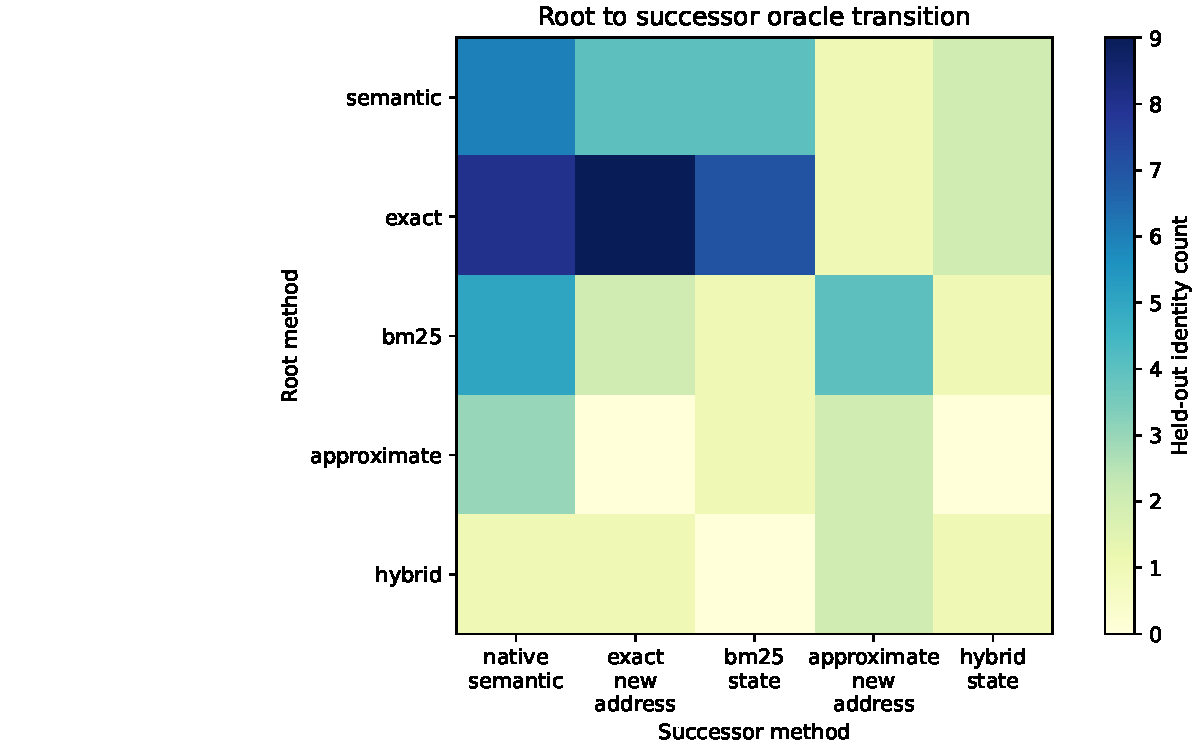
\includegraphics[width=.74\linewidth]{root_successor_transition_heatmap_expanded.pdf}
\caption{Per-example oracle root-to-successor transitions in the breadth cohort. The matrix is an opportunity diagnostic, not a deployable controller.}
\end{figure}

\begin{table}[H]
\centering
\scriptsize
\caption{Normalized efficiency for the highest-recall measured root--successor pair in each breadth cohort.}
\begin{tabular}{llrrrr}
\toprule
Dataset & Root $\rightarrow$ successor & $R_E$ & $P_E$ & $K/N$ & $K/E$\\
\midrule
QASPER & exact $\rightarrow$ exact address & .121 & .219 & .032 & 1.029\\
HotpotQA & approximate $\rightarrow$ semantic & .145 & .156 & .088 & .896\\
2Wiki & exact $\rightarrow$ semantic & .148 & .236 & .102 & .901\\
MuSiQue & BM25 $\rightarrow$ exact address & .086 & .278 & .050 & .327\\
\bottomrule
\end{tabular}
\end{table}
Complete recovery is zero throughout. Search comparisons and physical K/V activation remain separate costs.

\section{Interaction Details}
\label{app:interactions}
The corrected interaction run contains 4,608 rows and makes Top-2, Top-4, and Top-8 reachable by setting per-hop branch and beam widths to 1, 2, and 4. A pilot silently capped Top-8 and is excluded. Table~\ref{tab:matched-token-interactions} reports exploratory maxima at a fixed 128 routed tokens.

\begin{table}[H]
\centering
\scriptsize
\caption{Best late-layer channel at 128 routed tokens. $C_E$ is complete evidence recovery.}
\label{tab:matched-token-interactions}
\begin{tabular}{llrlrrr}
\toprule
Model & Dataset & Chunk & Best channel & Recall & Precision & $C_E$\\
\midrule
Qwen & HotpotQA & 16 & token $n$-gram & .938 & .266 & .875\\
Qwen & HotpotQA & 32 & bounded edit & .750 & .281 & .625\\
Qwen & HotpotQA & 64 & token $n$-gram & .875 & .438 & .875\\
Qwen & QASPER & 16 & token $n$-gram & 1.000 & .547 & 1.000\\
Qwen & QASPER & 32 & bounded edit & 1.000 & .812 & 1.000\\
Qwen & QASPER & 64 & exact & 1.000 & .938 & 1.000\\
SmolLM & HotpotQA & 16 & bounded edit & .938 & .328 & .875\\
SmolLM & HotpotQA & 32 & exact & .812 & .312 & .625\\
SmolLM & HotpotQA & 64 & token $n$-gram & 1.000 & .500 & 1.000\\
SmolLM & QASPER & 16 & hybrid & .958 & .438 & .875\\
SmolLM & QASPER & 32 & token $n$-gram & .958 & .625 & .875\\
SmolLM & QASPER & 64 & exact & 1.000 & .875 & 1.000\\
\bottomrule
\end{tabular}
\end{table}

\begin{figure}[H]
\centering
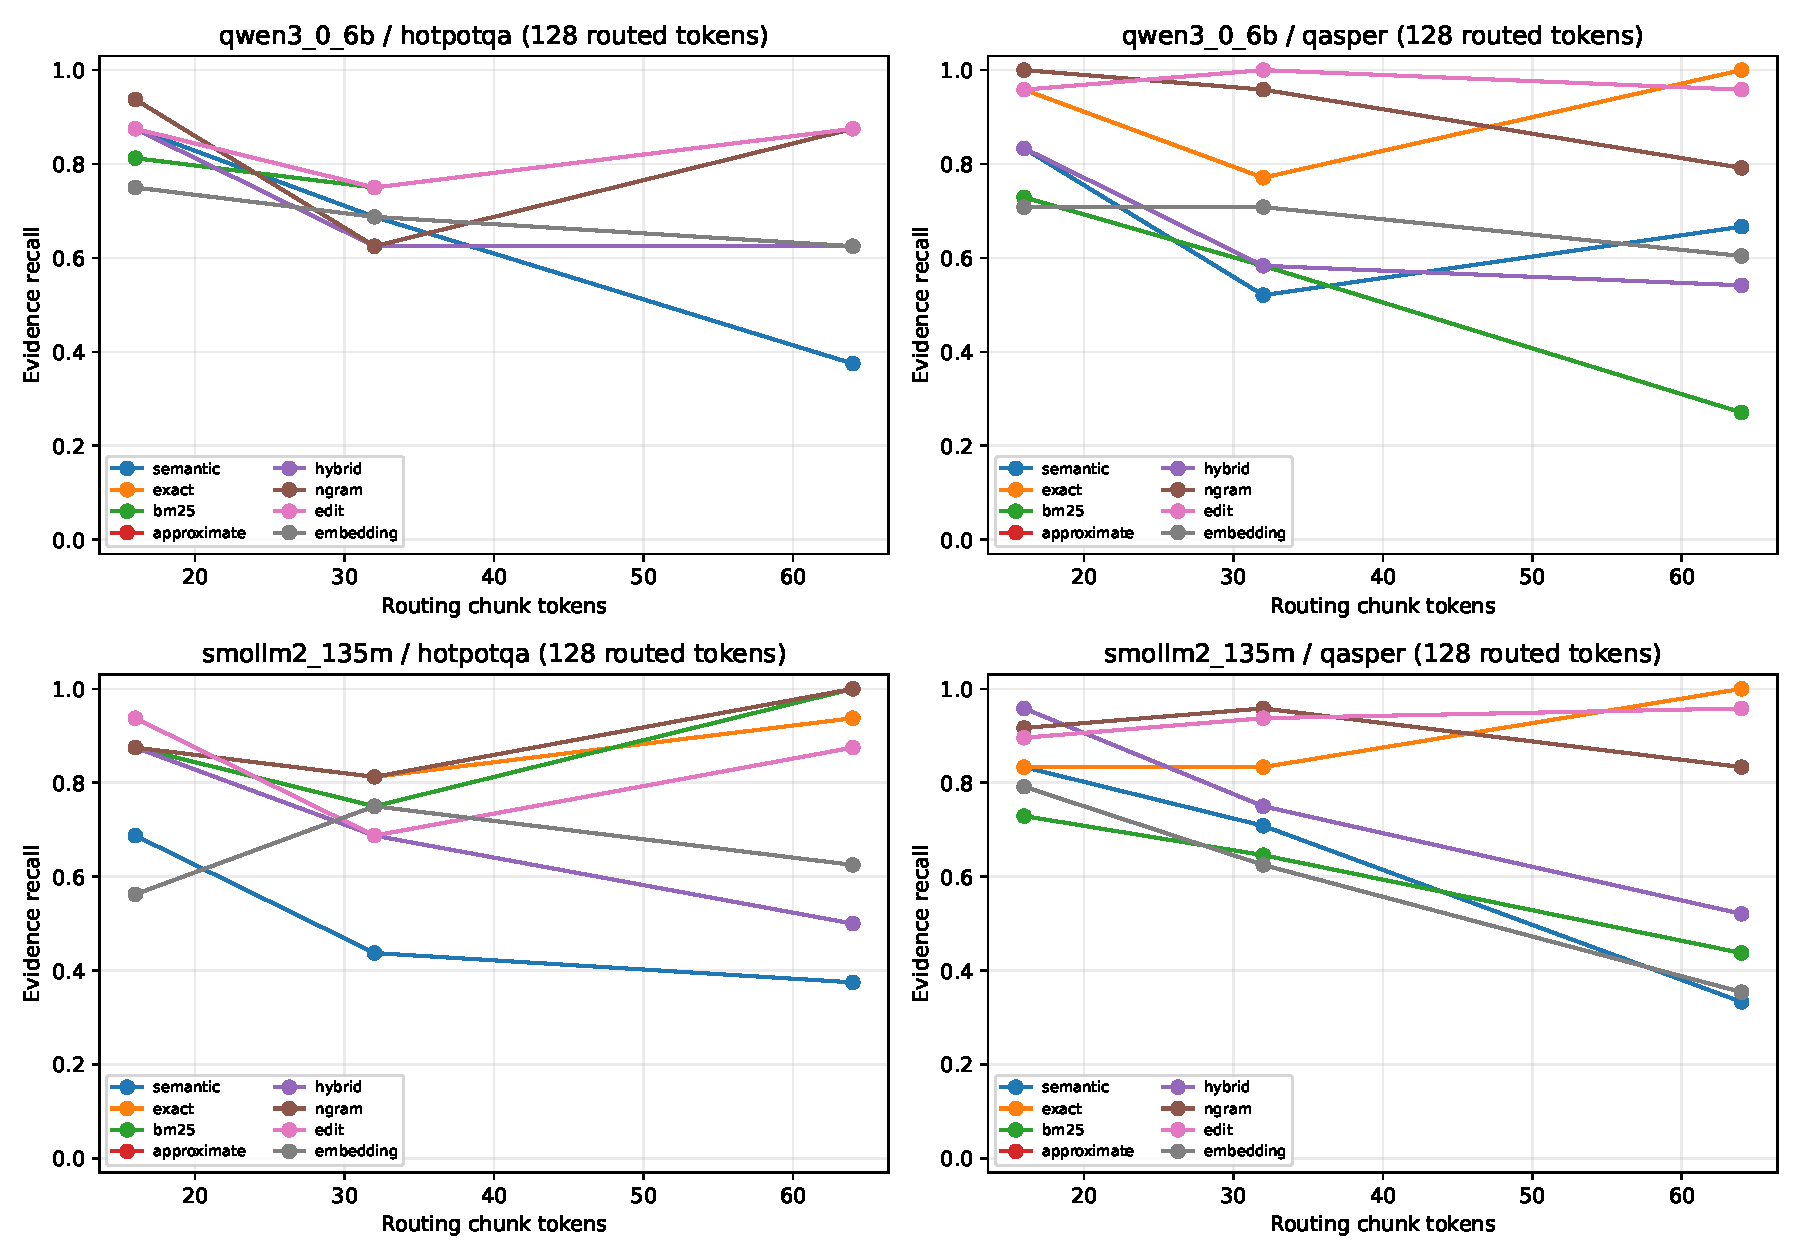
\includegraphics[width=.94\linewidth]{hybrid_interactions.pdf}
\caption{Evidence recall by representation and chunk size at 128 routed tokens. Ordering changes across dataset, model, and granularity.}
\end{figure}

\section{Artifact and Action Contract}
\label{app:contract}
The version-2 action specification freezes five root actions---semantic, exact, BM25, approximate, and hybrid---and five successor actions---native semantic, exact new address, BM25 state, approximate new address, and hybrid state. Each action names its implementation identifier, required state and indexes, legal parameters, confidence outputs, cost metrics, and known failures. Legacy names remain explicit aliases. The schema records whether a source experiment materialized K/V so that discovery-only artifacts cannot be mistaken for consumption measurements.

Committed artifacts include per-example retrieval rows, cohort-overlap audits, controller seed rows, paired retrieval and causal effects, a source-construction audit, physical K/V accounting, indexed latency and parity summaries, tokenizer perturbations, complete root--successor matrices, interaction rows, confidence diagnostics, and claim audits. The claim-to-artifact ledger is \path{docs/papers/paper2_6_hybrid_pra/CLAIM_LEDGER.md}; canonical results and implementation traces are under \path{docs/papers/shared/results/paper2_6_hybrid_pra/} and \path{experiments/paper2_6_hybrid_pra/}. This contract lets Paper~3.5 consume actions and observable fields without importing dataset identity or gold evidence into its controller.

\bibliographystyle{plain}
\bibliography{../shared/references}
\end{document}
